\documentclass[
  utf8,%     More capable input encoding than latin-1.
  % parskip,%  For vertical whitespace between paragraphs.  This comes down to more than just using parskip.sty, so it's better to use this class option.
  % S5MP % If you intend to really use margin paragraphs (not recommended!).
%  crop,%     Produce output with crop marks and paper size A4.  Liu-Tryck should like this.  Automatically adds information, including the physical page number, at the top of each page.
       %     Add option 'noInfo' to suppress the info at the top of each page when using option 'crop'.
  % Font options: 'kp' (default), 'times', 'lm'.  The KpFonts (loaded using 'kp'), is the most complete font among the provided options.  Among other, it supports slanted small caps.  See rtthesis.cls for more details regarding the font options.
  largesmallcaps,intlimits,widermath,% Good options to KpFonts.
  sharecounter,nobreak,definition=marks,%  See comments in the results chapter of this document for more information on these options!
  %numbers, % If you want to cite references by numbers, use this option.
  noparts% Use option 'noparts' if you do not make use of part divisions.
]{rtthesis}
\usepackage[T1]{fontenc}
\usepackage[bitstream-charter]{mathdesign}
\usepackage[font=footnotesize,labelfont=bf]{caption}
%\usepackage{listings}
%\usepackage[parfill]{parskip}
%\usepackage{float}
%\usepackage{graphicx}
%\usepackage[swedish]{babel}
%\usepackage[applemac]{inputenc}
\usepackage{mythesis}






\begin{document}
\selectlanguage{english}
\makeFrontPage
\frontmatter
\maketitle
\makeLibraryPage{The properties of free-standing cubic silicon carbide for optoelectronic applications are explored in this work. The main focus of the work is on boron doped cubic silicon carbide, which is proposed as a highly useful material in several optoelectronic applications. The material is grown using sublimation epitaxy and the doped material is grown homoepitaxially on nominally undoped seeds. It is characterized using the experimental setups of photoluminescence spectroscopy, Nomarski interference spectroscopy and absorption spectroscopy. 

I study seed growth of nominally undoped cubic material on hexagonal (4H) substrates, and the influence on the grown material from the different faces of the substrate. It is found that it is not possible under the explored conditions to completely cover the growth area with the cubic polytype on the carbon face, but it can be done reproducibly on the silicon face. Reasons for this are discussed. Different doping setups are also explored.

The influence on the material properties from growth conditions is explored. It is shown from absorption measurements that it is possible to grow boron doped cubic silicon carbide using this growth method, but optical microscopy studies show that the sample quality degrades with high doping concentrations. 

I explore the luminescence properties of the material. No boron related emission is found with either room temperature or low temperature photoluminescence spectroscopy. Reasons for this are discussed using results from absorption measurements and optical microscopy. 

}

\begin{abstract}[english]
  The properties of free-standing cubic silicon carbide for optoelectronic applications are explored in this work. The main focus of the work is on boron doped cubic silicon carbide, which is proposed as a highly useful material in several optoelectronic applications. The material is grown using sublimation epitaxy and the doped material is grown homoepitaxially on nominally undoped seeds. It is characterized using the experimental setups of photoluminescence spectroscopy, Nomarski interference spectroscopy and absorption spectroscopy. 

I study seed growth of nominally undoped cubic material on hexagonal (4H) substrates, and the influence on the grown material from the different faces of the substrate. It is found that it is not possible under the explored conditions to completely cover the growth area with the cubic polytype on the carbon face, but it can be done reproducibly on the silicon face. Reasons for this are discussed. Different doping setups are also explored.

The influence on the material properties from growth conditions is explored. It is shown from absorption measurements that it is possible to grow boron doped cubic silicon carbide using this growth method, but optical microscopy studies show that the sample quality degrades with high doping concentrations. 

I explore the luminescence properties of the material. No boron related emission is found with either room temperature or low temperature photoluminescence spectroscopy. Reasons for this are discussed using results from absorption measurements and optical microscopy. 


\end{abstract}
%\begin{acknowledgments}
  I wish to thank my supervisor, Jianwu Sun, for teaching me the experimental methods and for invaluable guidance in interpreting the results. I also wish to direct my thanks to Mikael Syväjärvi - thank you for taking me in as a master's student in your lab, and for the help and input in planning my work and writing this thesis. I really appreciate having had the opportunity to be a member of your group during this time. Finally thank you also to Valdas Jokubavicius and Xinyu Liu for your support and guidance in the lab. 

  \addvspace{1em}
  \begin{flushright}
    \textit{%
      Linköping, Juni 2015\\
      Mattias Jansson%
    }
  \end{flushright}
\end{acknowledgments}

\tableofcontents
%\begin{notation}% Passing the option "old" to the notation environment will redefine the notationtabular environment so that it produces an old style LaTeX tabular instead of a ctable.sty style tabular.
  \centering

  \begin{notationtabular}{Några mängder}{Notation}{Betydelse}
    $\naturals$ & Mängden av naturliga tal \\
    $\reals$ & Mängden av reella tal \\
    $\complexes$ & Mängden av komplexa tal \\
  \end{notationtabular}

  \begin{notationtabular}{Förkortningar}{Förkortning}{Betydelse}
    \abbrARMA\index{ARMA@\abbrARMA!abbreviation} & Auto-regressive moving average \\
    \abbrPID\index{PID@\abbrPID!abbreviation} & Proportional, integral, differential (regulator) \\
  \end{notationtabular}
\end{notation}


\mainmatter

%-*- mode: LaTeX; -*-

\chapter{Introduction}
%This thesis deals with SiC 
%Good properties when it comes to stability
%Used in power electronics, radiation (space - Citation needed!)

%SiC is a semiconductor
%Exists in a number of different polytypes
% This thesis deals with the cubic polytype
%One of the most common polytypes

% Difficulty in fabricating 3C with good quality
% Using sublimation epitaxy (FSGP)

% The band gap of 3C is good for solar cell applications
% And for water splitting
% Using doping to enhance the properties

% This thesis deals with examination of optical properties 
% List the characterization methods

% Describe the chapters

Silicon carbide (SiC) is a semiconductor which has attracted interest in research and industry since the 19:th century, when it was first fabricated and used as an abrasive \cite{Acheson1893}. SiC has been found to be a very stable material. It exhibits a high chemical inertness \cite{Hume1941}, and is currently commonly used in high power, temperature and radiation applications due to its ability to survive in such environments \cite{J.B.CASADYandR.W.JOHNSON1996}. 

SiC is a material which exists in a large number of different polytypes, the most common of which are hexagonal, cubic and rhombohedral. The work described in this thesis deals with the cubic polytype, denoted \emph{3C-SiC}. This is one of the structurally most simple polytypes, and the only cubic one. Compared to the hexagonal counterparts 4H- and 6H-SiC, the 3C-SiC polytype has for a long time been difficult to fabricate in good quality and large volume, and is therefore less studied than the hexagonal types. Recently a method of fabricating good quality free standing cubic material using sublimation growth has been reported \cite{Jokubavicius2014}. The method has been used to grow the samples used in the work described in this thesis. With this method it is possible to grow free-standing 3C-SiC, which means that the material is thick enough to exist on its own after mechanically polishing away the 4H-SiC substrate. 

Cubic SiC has many interesting material properties. It has a higher electron mobility compared to the common hexagonal polytypes \cite{Schoner2006}. It has also attracted attention as a transistor material, since it can can achieve a low number of interface defects in such structures \cite{Anzalone2015}. One application for which 3C-SiC is well suited is the use of boron doped 3C-SiC in an intermediate band photovoltaic solar cell. This is suitable for 3C-SiC due to its band gap size of 2.36 eV, together with the binding energy of boron as an acceptor in the material, which is almost ideal for photovoltaic cell material. This would give a significant increase in photovoltaic cell efficiency compared to the conventional single junction alternative \cite{Richards2003},\cite{Luque1997}. Another proposed application of 3C-SiC is as a photo-electrode in a photoelectrochemical cell used for water splitting \cite{Kato2014,Yasuda2012}, where solar energy is used in the decomposition of water into hydrogen and oxygen gas. 

This thesis describes the growth and optical characterization of free-standing cubic silicon carbide, which is vital for the realization of 3C-SiC optoelectronic applications such as the intermediate band solar cell and the water splitting electrode. The work carried out in this project can be divided into two parts. The first part deals with growth of the boron doped material which is to be investigated. This parts includes growth of nominally undoped seeds and growth of the boron doped material. The second part deals with characterization of the grown samples. Characterization has been carried out using photoluminescence spectroscopy, absorption spectroscopy and optical microscopy. 

The thesis is divided into several chapters as follows: chapter \ref{sec:sic} gives an introduction to silicon carbide, its structure and properties. Chapter \ref{sec:growth} describes the process of growing the material. Both growth of undoped and boron doped material is described here. In chapter \ref{sec:characterization} a description of the different characterization methods is given, together with a theoretical description of what the measurements can tell about material properties. Chapter \ref{sec:experimental} describes how the experiments were done and chapter \ref{sec:results} describes the results obtained from the experiments. The results are discussed in chapter \ref{sec:discussion}. Chapters \ref{sec:conclusion} and \ref{sec:future} discuss what has been learned about the material and how the work should be continued in the future. 




































\label{sec:introduction}

%-*- mode: LaTeX; -*-

%Consists of Si and C atoms, crystal. (Arranged periodically)
%There exists many (Citation?) different kinds of polytypes
%Polytypes can be thought of as stacking sequence of hexagonal layers
%Base is one C and one Si
%Si and C faces, what is that? [Do I need this?]
%If I do anything on bulk, then I should discuss planes here. (Since the goal is to have (100) plane).

%The atoms are bonded together by covalent bonds.
%The band structure is shown...
%Indirect band gap of...
%Phonons

%Some relevant properties
%Mobility
%Dielectric constant

%Nitrogen as background doping
%Possible acceptors are
%Boron doping gives good band diagram as seen...


\chapter{An introduction to silicon carbide}
\label{sec:sic}
This chapter describes the properties of SiC which are relevant to this thesis. Section \ref{sec:crystal_structure} describes the atomic arrangement in the material, and some different arrangements are discussed. Section \ref{sec:band_structure} discusses the energy band structure of 3C-SiC. Finally section \ref{sec:doping_in_3C} describes the mechanism and some effects of doping in 3C-SiC. 

\section{Crystal structure}
\label{sec:crystal_structure}
Silicon carbide is a crystalline material consisting of silicon and carbon atoms. The crystalline nature of the material means that the atoms are arranged in a periodically repeating structure called a \emph{lattice}. For given chemical elements there may be several different ways to arrange the atoms in a lattice, i.e. different chemical compounds of the same types of atoms. This is called \emph{polytypism}, where the different lattice structures are called \emph{polytypes} of the material. SiC has a large number of different polytypes - there are more than 250 known polytypes of SiC \cite{Cheung2006}. The different polytypes can be described as different stacking orders of layers of atoms \cite{Mirgorodsky1995}. Figure \ref{fig:hex} shows one such layer. The depicted layer is the (111) surface. Here each circle symbolizes one carbon and one silicon atom, displaced a small distance from each other. This pair of atoms is called the \emph{base} of the crystal. 

\begin{figure}[h]
\begin{center}
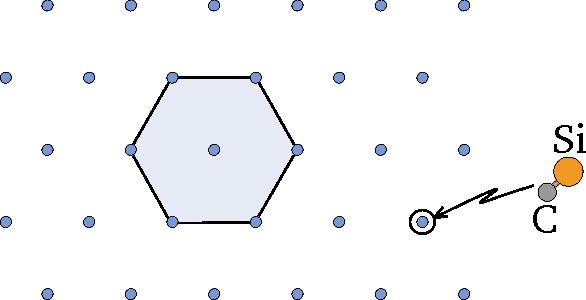
\includegraphics[scale=1]{lattice2.pdf}
\caption{Atomic arrangement of the atoms in each (111) layer. Here each sphere corresponds to one carbon and one silicon atom, as shown by the arrow. 
\label{fig:hex}}
\end{center}
\end{figure}

The marked hexagon in figure \ref{fig:hex} marks an area of the crystal plane which can be used to define the different polytypes, where the polytypes are defined by the placement of the base atoms in this area in different layers. Figure \ref{fig:poly} shows these stacking sequences for three of the most common polytypes. The depicted orders of the layers refers to one period in the periodic structure. The names for the different polytypes are stated at the top of the figure. The digit in the name refers to the number of layers of a period and the letter denotes the crystal symmetry. The letter \emph{H} denotes the hexagonal polytypes, whereas \emph{C} stands for the cubic polytype. Another common polytype is the 6H-SiC, which thus is a hexagonal structure with a period of six base layers. It should be noted that the 2H structure is the wurtzite structure and the 3C is the zincblende structure. The unit cell of the zincblende, or 3C, crystal has a lattice constant of $\mathrm{a} = 4.35$ Å \cite{Bimberg1981}. 


%\begin{figure}[h]
%\begin{center}
%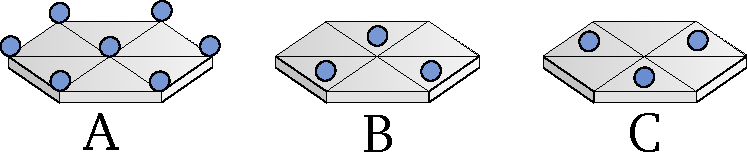
\includegraphics[scale=0.7]{hex5.pdf}
%\caption{Different atomic placements for the layers
%\label{fig:stacking1}}
%\end{center}
%\end{figure}


\begin{figure}[h]
\begin{center}
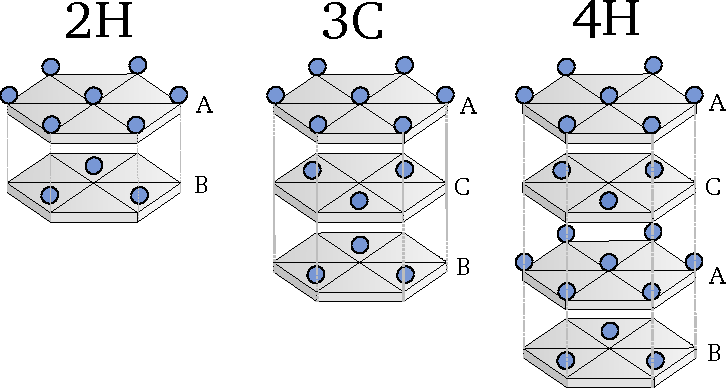
\includegraphics[scale=0.8]{poly.pdf}
\caption{Stacking order for the three most simple polytypes. 
\label{fig:poly}}
\end{center}
\end{figure}

\section{Band structure}
\label{sec:band_structure}
%The atoms are bonded together by covalent bonds.
%The band structure is shown...
%Energy gap - no available energy states
%valence and conduction bands
% Indirect band gap value
	%Change of k, momentum
%Direct band gap value. 

In SiC the atoms are bonded together with covalent bonds [Citation Zumdahl: Chemistry?] into a crystal. When the atoms are bonded together, the energy levels for the electrons in the material are defined by the material and lattice structure. This means that all materials have characteristic energy levels. When many atoms are bound together, as is the case in crystals, the discrete energy levels for the electrons in the atoms merge together to form continuous bands, called energy bands. 

The band structure for 3C-SiC is shown as a band diagram in figure \ref{fig:band}. In this figure, each curve describes allowed energies for the electrons, and the spaces in between the curves are not allowed. The x-axis shows different points in reciprocal space, or \emph{k-space}. The marked points are specific points in the first brillouin zone of k-space, and the intermediate intervals form straight lines between the points. This figure has been obtained using the approximate method of pseudopotentials, as described in \cite{Aourag1994}. Here the zero point energy has been chosen to be at the $\Gamma$-point in k-space. 

The grayed area in the figure is the \emph{band gap} of the material, since there are no allowed electronic states in this area. The band with lower energy than the band gap is called the valence band, and the band with higher energy is called the conduction band. 3C, as is characteristic for semiconductors, has the fermi level in the middle of the band gap. This means that at the temperature of 0 K, all electrons will be in the valence band, and the conduction band will be unoccupied. When the conduction band is unoccupied the material will not be able to conduct electricity. If the temperature is raised above 0 K there will be some occupation of the conduction band and some electrical conduction will be able to occur. With a higher temperature there will be more electrons in the conduction band and thus a higher conductivity of the material. 

\begin{figure}[h]
\begin{center}
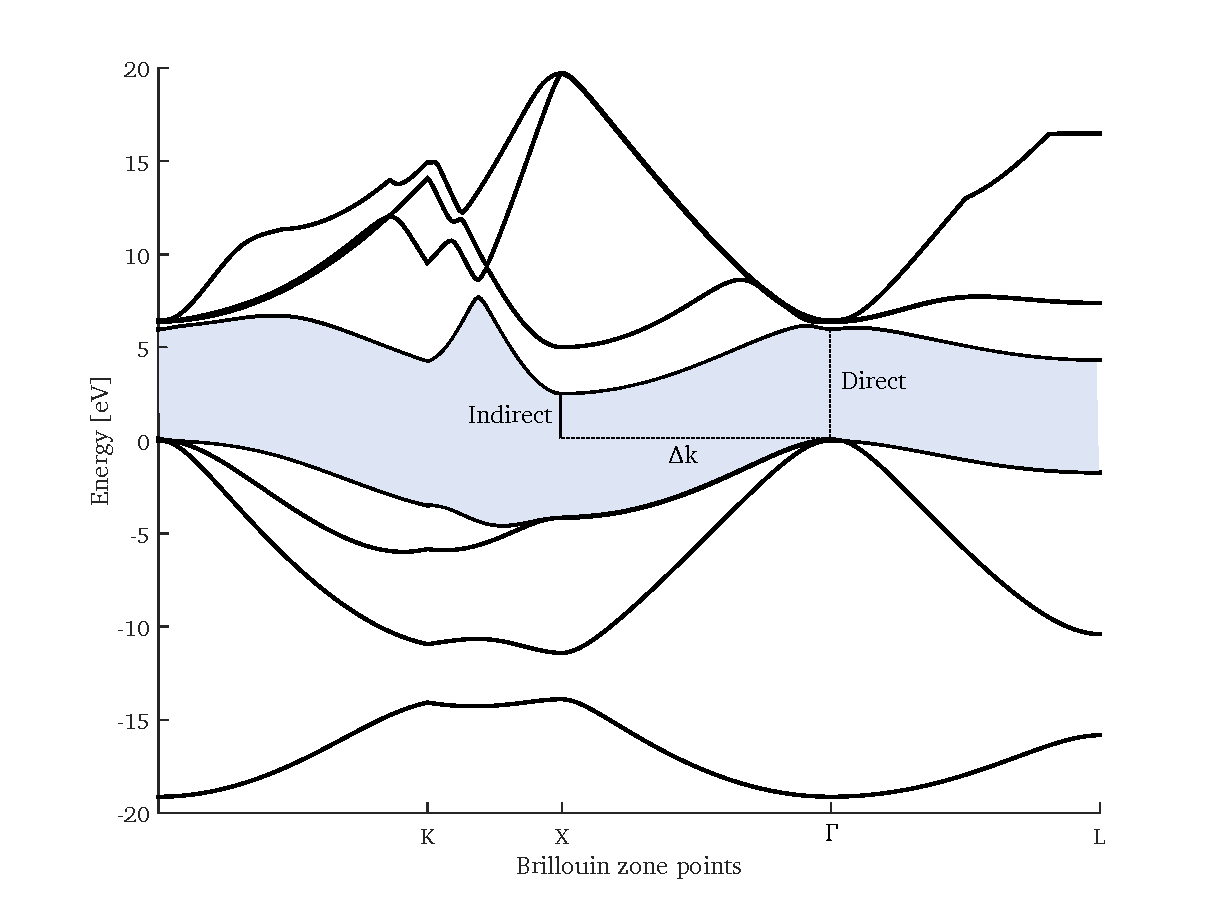
\includegraphics[scale=0.6]{band_diagram2.pdf}
\caption{The band diagram of SiC at ambient conditions for different positions in the Brillouin zone. The indirect and direct band gaps are marked in the figure. The marked area is the band gap. The energy levels have been obtained using the pseudopotential method, as described in \cite{Aourag1994}.
\label{fig:band}}
\end{center}
\end{figure}

In the figure \ref{fig:band} it can be seen that the smallest energy difference between the valence and conduction bands is between the $\Gamma$-point in the valence band and the X-point in the conduction band. This difference is called the \emph{band gap}. The difference between the $\Gamma$- and X-points is called the indirect band gap, while the difference between the values at the $\Gamma$-point is called the direct band gap, as illustrated in the figure. These values are given in table \ref{tab:eg}. The value for the indirect band gap at room temperature is taken from the simulation, whereas the latter values are taken from literature. 

\begin{table}[h]
\caption{Values for the indirect and direct band gap energies. The indirect values are given both for room temperature and low temperature, as this will be of value later in the thesis.}
\label{tab:eg}
\begin{center}
\begin{tabular}{ l c r }
  \hline                       
  \hline       
  \vspace{1mm}
    $\mathrm{E_{g,indirect}}$  (300 K) & $\mathrm{E_{g,indirect}}$ (2 K) & $\mathrm{E_{g,direct}}$  (300 K)\\
    \hline
  2.36 eV & 2.42 eV \cite{Bimberg1981} & 6.00 eV \cite{Dalven1965}\\
  \hline  
\end{tabular}
\end{center}
\end{table}

When an electron makes the indirect transition from the valence to the conduction band the energy is increased by E$_\mathrm{g}$, and the k-value is changed, as indicated by $\Delta \mathrm{k}$ in figure \ref{fig:band}. This change of k-value implies a change in momentum of the electron, since k and momentum p is related by

\[p = \hbar k,\]

\noindent where $\hbar$ is Dirac's constant. This is of importance when studying interaction between the material and light. Photons are capable of providing the energy needed to transit from the valence to the conduction band, but cannot provide the change of momentum needed. The law of conservation of momentum requires the total momentum of the system to be preserved during the transitions. The extra momentum can however come from interaction with phonons. 

The phonon energy spectrum has four ground modes, since there are two different kinds of atoms in the material. There are the acoustic and optical phonon modes. Theoretical calculations of the phonon dispersion curves for 3C have been done by Karch et al. \cite{Karch1994}. They show the four modes: TA, LA, TO, LO, and give the wavelength for each mode. The transition in k-space for the indirect transition is between the $\Gamma$- and the X-points, hence it is of interest to know which phonon wavelengths and energies this corresponds to.  Table \ref{tab:phonons} shows these computed wavelengths and the corresponding energies, which have been calculated using the fact that

\[E_{meV} = \frac{hc(\frac{1}{\lambda_{cm}})}{e}\times 10^5,\]

\noindent where h is Planck's constant, c is the speed of light and e is the elementary charge. 

\begin{table}[h]
\caption{Inverted wavelengths and energies for the $\Gamma$-X tranistion. Values for $\lambda$ from \cite{Karch1994}.}
\label{tab:phonons}
\begin{center}
\begin{tabular}{ l l l }
  \hline                       
  \hline       
  \vspace{1mm}
    Mode  & $\lambda^{-1} [\mathrm{cm}^{-1}]$  & E [meV]\\
    \hline
  TA &  368 & 45.6\\
  LA &  637 & 79.0\\
  TO &  760 & 94.3\\
  LO &  829 & 102.9\\
  \hline  
\end{tabular}
\end{center}
\end{table}





%\section{Some properties}
%\label{sec:}




\section{Doping in 3C}
\label{sec:doping_in_3C}

% Doping is when an atom is replaced
% Donors and acceptors, number of valence electrons. 
% Donors can donate, acceptors accept, as seen in fig. 
	% Nitrogen doping, more electrons
	% Ionization energy 
	% Difficult to avoid
	
	% Some possible acceptors
	% And their energies
	% Refer to section about B-doped solar cells. 
% Doping can be achieved...
% Problems which can occur with doping are...


Doping is a way to change the electronic structure of a material by substituting some of the native atoms with a foreign element. In the case of SiC this means that either silicon or carbon is replaced by some other element. How the band structure of the material is changed depends on which material is introduced to the crystal. By choosing the dopants it is possible to tailor the band structure to create various new properties of the material. 

An important factor for how the band structure is changed is the number of valence electrons in the introduced element, compared to the element it replaces. Silicon and carbon both have four valence electrons, creating four bonds to its neighbouring atoms in the crystal. The electrons are strongly bound to the atomic nuclei, requiring energy corresponding to the band gap to free one electron. If one silicon or one carbon atom is replaced by an element with five valence electrons however, the additional electron is not as strongly bound to the nucleus and can easily release an electron to the conduction band. This is called a \emph{donor} atom. Similarly if an atom with only three valence electrons is introduced to the crystal, it can readily bind an electron from the valence band, creating an electron deficiency, or \emph{hole} in the valence band. This is called an \emph{acceptor} atom. Figure \ref{fig:dopant_band} shows a simplified band diagram with a donor and an acceptor level. The donor level donates an electron to the conduction band by supplying the energy $\mathrm{E_D}$ to the electron. The acceptor accepts an electron from the valence band by supplying the energy $\mathrm{E_A}$. The energy required to supply the material with one carrier from a dopant level is called the \emph{binding energy} (or \emph{ionization energy}) of the dopant. 

\begin{figure}[h]
\begin{center}
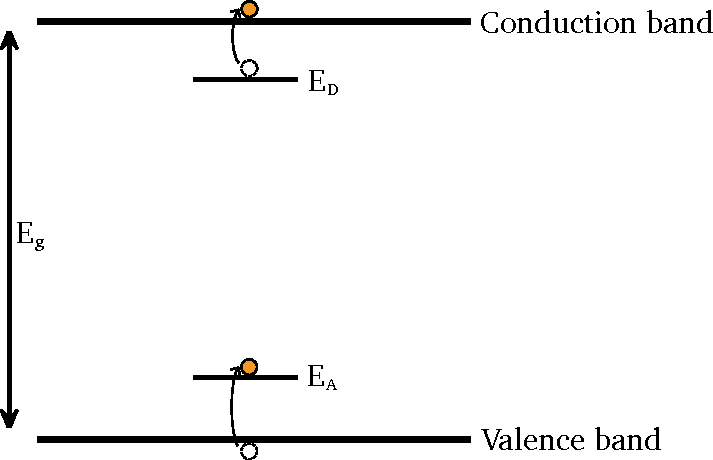
\includegraphics[scale=0.6]{doped_band1.pdf}
\caption{Two new energy levels are introduced by doping. 
\label{fig:dopant_band}}
\end{center}
\end{figure}

\subsection{Donors}
% What does it replace, Si or C?
Since silicon and carbon both have four valence electrons, a donor atom in SiC must have five or more electrons. One common donor is nitrogen, which has five valence electrons. This means that each added N-atom can supply the conduction band with one electron. A material with more donors than acceptors is said to be an \emph{n-type} material. Freitas et al. have measured the binding energy of nitrogen in 3C, and found it to be 54 meV \cite{Freitas1988}. This means that the lowest N-level is 54 meV below the conduction band. 

N-doping can be achieved intentionally by fabricating the material in a nitrogen atmosphere, but nitrogen always present in FSGP-grown material even at dynamic vacuum conditions \cite{Sun2012b}. This means that material grown by this method is generally n-type. The n-type material can also be created by other elements in group five. Reports of doping with As, P and Sb exist, but are far less common than N-doping \cite{Rao1999}. 

\subsection{Acceptors}
% What do they replace, Si or C?
Acceptor atoms need to have fewer valence electrons than silicon and carbon, which is why group three elements are the most common. These include boron and aluminum, which have the binding energies 257 meV \cite{Freitas1988} and 735 meV \cite{Richards2003} respectively. A material with more acceptors than donors is said to be \emph{p-type}. Table \ref{tab:dopants} summarizes the different dopant energy levels. 

\begin{table}[h]
\caption{Binding energies for some of the most common SiC dopants.}
\label{tab:dopants}
\begin{center}
\begin{tabular}{ l l l r}
  \hline                       
  \hline       
  \vspace{1mm}
    Element  & Dopant type & E$_{D/A}$ [meV] & Reference\\
    \hline
  N &  Donor & 57 & \cite{Freitas1988}\\
  B &  Acceptor & 735 & \cite{Richards2003}\\
  Al &  Acceptor & 257  & \cite{Freitas1988}\\
  \hline  
\end{tabular}
\end{center}
\end{table}

The B-doping energy level is of particular interest for photovoltaic applications, where the binding energy is ideal for the impurity photovoltaic solar cell. This is described in more detail in chapter \ref{sec:ipv}. 
\\ 

\noindent 
There are several ways to create doped materials. It can be done by ion implantation, where ions are accelerated to high energies and then made to collide with the undoped material \cite{Rao1999}. It can also be done as the material is grown, by including the doping element in the ambient. The first method has several advantages: it can be done with good control over doping density and it is possible to select only certain areas of the material to dope. The latter method is done \emph{in situ}, so it requires no additional equipment. It is also not as prone to create defects as the ion implantation method is, where annealing is often required after implantation. In the work described in this thesis, the method of doping is to include the doping material during the growth. This method is described in more detail in chapter \ref{sec:growth}. 

During doping some of the native atoms are replaced. This will have effects on the quality of the produced material. Different elements have different atomic radii, so replacing one atom by one of a different element will create some strain in the material. This may lead to defects in the material. 






































%-*- mode: LaTeX; -*-

\chapter{Growth techniques}
This chapter describes the growth technique. 

%-*- mode: LaTeX; -*-

%Introduction to characterization
	%Optical properties and morphology
	%Electrical properties are also of interest, but beyond scope
%Absorption
	%General about absorption and transmission of semiconductors
	%Describe setup in general
	%How to compute coefficient and band edge
%PL measurements
	%General about excitation and recombination, luminescence 
	%Describe the setup
		%RT vs LT
	%How to infer the band structure from the PL-spectrum
	%Other properties that can be found from PL
%Water splitting measurements 
	%General about water splitting
	%The setup
	%Oxidation of electrodes
%Optical microscopy
	%Nomarski interference 
	%Reflection mode
\chapter{Characterization techniques}
\label{sec:characterization}
To investigate the material properties after growth, the samples must be characterized. There are many established techniques to do this. This chapter gives a description of the characterization techniques used to obtain the results in this thesis. This thesis focuses partly on the morphology of the samples and partly on the optical properties of the grown samples. The specifics of the experiments performed are given in chapter \ref{sec:experimental}.

%-*- mode: LaTeX; -*-

\section{Absorption measurements}
Here will follow a description of how the absorption measurements were done. 
%-*- mode: LaTeX; -*-
%PL
	%General about excitation and recombination, luminescence 
		%On phonons and replicas
		%On the method of finding stress using phonons
		%On doped materials, and finding their levels using PL
		%On Excitons, binding energies
			%Bound excitons and free excitons
			
	%Describe the method of finding the dopant concentration
			
		
	%Describe the setup
		%Laser and optics
		%Spectrometer
		%RT vs LT

	
\section{Photoluminescence spectroscopy}
\label{sec:pl}
Photoluminescence (PL) spectroscopy is a very powerful tool in optical characterization of semiconductors. It is a non-invasive and fast technique. PL is similar to absorption spectroscopy in that a light source is aimed at the sample to induce electron excitations. As an electron radiatively recombines with a hole, a photon is emitted. These emitted photons are called the \emph{luminescence} of the sample, and is what is measured in PL spectroscopy. 


%Figure \ref{fig:pl1} shows a schematic of the method of generating luminescence. As the laser beam (A) hits the sample (B), photoluminescence (C) is generated. As not all laser light is absorbed, some of the light reflects away form the sample (D). 

%\begin{figure}[h]
%\begin{center}
%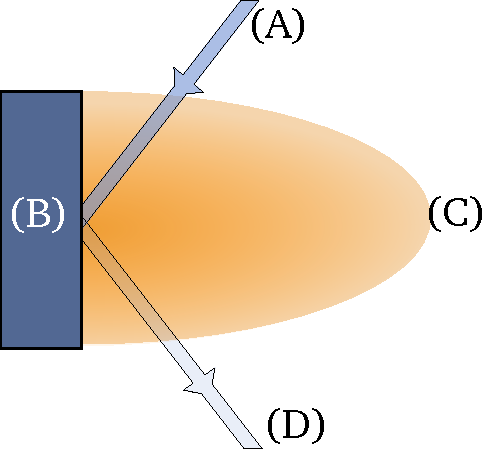
\includegraphics[scale=0.5]{PL1.pdf}
%\caption{Photoluminescence induced from a sample by a laser beam. 
%\label{fig:pl1}}
%\end{center}
%\end{figure}

The process of excitation and recombination is shown in figure \ref{fig:pl2}, where a photon is captured (a) and generates an \emph{electron hole pair (EHP)} (b). The EHP then recombines and emits a photon of energy corresponding to the band gap, E$_g$ (c). 

\begin{figure}[h]
\begin{center}
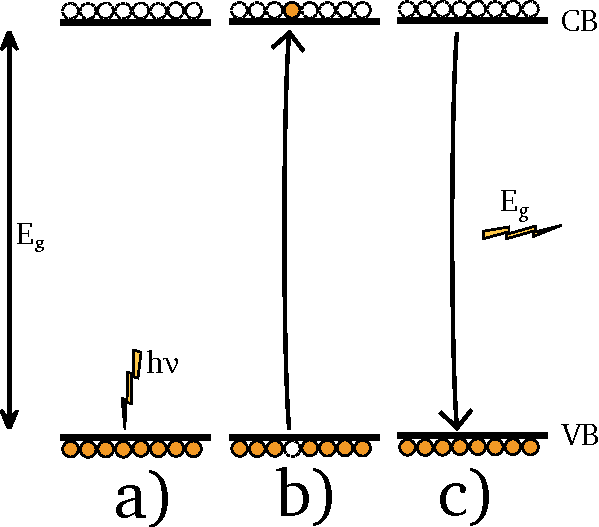
\includegraphics[scale=0.6]{PL2.pdf}
\caption{An EHP is generated (b) by capture of a photon (a) with energy $h\nu$, which must be greater than or equal to the band gap energy. The EHP recombines to emit a photon of energy E$_g$ (c).
\label{fig:pl2}}
\end{center}
\end{figure}

To generate an EHP by a transition between the valence and conduction bands, the energy of the light must be greater than the band gap. This is in accordance with the principle of conservation of energy. The laser must be chosen accordingly. Not only the energy is conserved in this process, but as is the momentum. Since SiC is an indirect semiconductor (see figure \ref{fig:band}), an electron moving across the band gap has a change in momentum. The light momentum is far too small to compensate for this change. To allow the EHP to be generated, the change in momentum is contributed by phonons. As the transition occurs, a phonon is either created or annihilated. The phonon energies for the different modes in 3C-SiC are given in section \ref{sec:band_structure}. The phonons show in PL spectra as lines with energies slightly smaller than the value of the actual electron energy transition, called the \emph{zero phonon line (ZPL)}. The phonon lines are called \emph{phonon replicas}. 

The phonon replica lines can be used to investigate the biaxial stress in the material. The PL intensity of the transverse optical and longitudinal acoustic modes should be the same if the material is without internal stress. Hence the ratio 
\[\frac{I_{\mathrm{LA}}}{I_{\mathrm{TO}}}\]
should be near unity in good quality samples \cite{Sun2012b}. Here I$_\mathrm{LA}$ and I$_\mathrm{TO}$ are PL intensities of arbitrary units. The phonon lines can aslo be used to estimate the doping concentration of a dopant. Camassel et al. have introduced a method where the full width at half maximum (FWHM) value of the TA-peak is used for this purpose. They show that the concentration of nitrogen donors in the sample is proportional to the FWHM, $\Gamma$, through the formula
\begin{equation}
\label{eq:fwhm}
\Gamma_\mathrm{TA} = A[N]^{1/n}.
\end{equation}
Here A and n are constants and [N] denotes the concentration on nitrogen donors. This method has however not been validated for acceptor type impurities. 


If doping levels are introduced in the band structure, then transitions can occur between such levels and the bands. In this case there will be another set of ZPL and phonon replicas at the new transition energy. The band structure can thus be inferred from the PL spectrum. 

As the EHP are generated, the electron and hole will interact with each other through the Coulomb force if they are near enough to each other. Due to their charge difference, they will start to orbit each other. This is called the \emph{exciton} quasiparticle. The energy of recombination of an exciton is slightly shifted from a normal recombination of a EHP, due to the potential energy from the Coulomb interaction. At room temperature the thermal energy from the ambient is generally high enough to split the exciton into a free electron and hole, so the excitons are not seen in the PL spectrum. At very low temperatures there is not enough energy to split the exciton, so the PL spectrum shows this shift in the recombination energy attributed to the Coulomb interaction. Some excitons can freely move in the sample, but some excitons bind to impurities in the sample. There is a small energy difference in the free and bound excitons attributed to the binding energy to the impurity. It is thus possible to distinguish from the free and bound excitons in the PL spectrum. 

The PL setup can be described as follows. An optical setup is used to focus a laser beam on a sample. The emitted photoluminescence passes through another optical setup and is focused into a spectrometer. The spectrometer separates the incident light by wavelength, generally by the use of a grating. Photons with a given wavelength can now be collected by a photomultiplier tube or a CCD camera, and the photon intensity for the wavelength spectrum can be computed. Light is captured during a set time (generally ranging between seconds to minutes depending on the sample and setup). 

The sample can be placed in a cryostat to measure the luminescence at low temperature, or measurements can be performed in room temperature. Various types of cryostats exist, generally using either liquid nitrogen or helium. In this work results have been obtained using room temperature measurements and by the use of a liquid helium cryostat. 







































%%-*- mode: LaTeX; -*-
%Water splitting measurements 
	%General about water splitting
	%The setup
	%Oxidation of electrodes


\section{Photocurrent through water splitting}
\label{sec:photocurrent}
To do.
































%-*- mode: LaTeX; -*-
%Optical microscopy
	%Nomarski interference 
	%Reflection mode

	
\section{Nomarski interference contrast microscopy}
\label{sec:nomarski}

Nomarski interference contrast microscopy, also known as differential interference contrast microscopy, is a version of optical microscopes designed to be able to investigate the inside of samples. The method utilizes the polarization of light to give slightly different light paths depending on where in the sample the light passes. The setup is shown in figure \ref{fig:nomarski}.

\begin{figure}[h]
\begin{center}
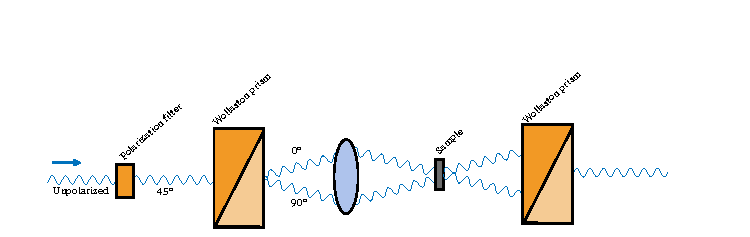
\includegraphics[scale=1]{sin.pdf}
\caption{A schematic of the Nomarski microscope setup. The light passes through the setup from the left to the right. 
\label{fig:nomarski}}
\end{center}
\end{figure}

The light is initially unpolarized. After passing a 45$^\circ$ polarization filter, the light enters a Wollaston prism. This prism will split the light in different directions depending on the polarization, creating two diverging beams. One beam will have light polarized in the 0$^\circ$ direction and the other in the $90^\circ$ direction. These two beams are focused on the sample by a lens, but made to hit the sample at slightly different positions. This will give the light beams slightly different paths through the sample. As the beams leave the sample they will enter another Wollaston prism, which will merge the two beams into one, and give the beams the same polarization, 135$^\circ$. If the beams have travelled different lengths in the sample, or if the sample composition has varied between the two paths, then the beams will be slightly out of phase. This phase difference will through interference between the beams lead to optical contrast.

One possible use for the Nomarski microscope is to detect different thickness in the sample. It can also be used to detect  sample composition difference, if the compositions have different refractive indexes. An example would be if a 3C-SiC sample has some hexagonal inclusions, then these will give contrast in the microscope since the hexagonal and cubic polytypes have slightly different refractive indexes. 








































\label{sec:characterization}
	%\subsection{Nomarski microscopy}
	%\subsection{Photoluminescence spectroscopy}
	%-*- mode: LaTeX; -*-

\section{Absorption measurements}
Here will follow a description of how the absorption measurements were done. 
	\label{sec:absorption}
	%\subsection{Hydrogen generation measurements}
	
%-*- mode: LaTeX; -*-

\chapter{Experimental setup}
\label{sec:experimental}
In this chapter, the details of the experimental setups are explained. The chapter is divided into two parts. The first part describes how the samples were grown and prepared. The second part describes details on the experimental setups for the characterization experiments. 

\section{Growth and sample preparation}
\label{sec:experimental:samples}
All samples used in this work are grown using sublimation growth, as described in section \ref{sec:growth:fsgp}. The nominally undoped samples are grown using two layers of polycrystalline SiC source material. 4H-SiC substrates with 4$^\circ$ off axis surface were used for undoped growth. The samples were cut along the (0001)-plane, with an off-axis angle towards the <11$\overline{2}$0> direction. The substrates were chemically cleaned before growth. Both the carbon and the silicon face of the 4H-SiC substrates were used during growth of undoped samples. 

The doped samples were grown using either direct or indirect doping methods, as described in section \ref{sec:growth:fsgp:doping}. The source material for doped growth was doped polycrystalline SiC, doped with boron concentrations in the order of $10^{18}$, $10^{19}$ or $10^{20}$ cm$^{-3}$. This was used together with a piece of undoped source material. The doped samples were grown either homoepitaxially on an unintentionally doped seed, or heteroepitaxially on the silicon face of a 4H-SiC 4$^\circ$ off-axis substrate. 

A piece of tantalum foil was placed in the bottom of the crucible for use as a carbon getter during growth of all samples. The source and substrate or seed were separated by a 1 mm thick graphite spacer for all samples. The substrate was held in place on the spacer by a graphite plate placed on top. All samples were grown at pressures in the order of $10^{-4}$ to $10^{-5}$ mbar, varying during the growth process. A vacuum pump was connected to the reactor and running continuously during growth. The temperature and growth time were varied between samples, and are given for individual samples in section \ref{sec:results}. The temperature was changed by varying the power supplied by the RF generator to the copper coil. The reactor setup is described further in section \ref{sec:growth:fsgp}. Care was taken to place the insulating foam containing the crucible in the same position in the reactor for each run. 

After growth the reactor was cooled in vacuum, by instantly setting the RF-generator to 0 W when the growth time was over. Cooling time was reduced by the use of a fan placed outside of the reactor. Optical microscopy images were done on as-grown samples, but any other characterization was done after chemically cleaning the samples. Cleaning was done with acetone and ethanol followed by H$_2$O:NH$_3$:H$_2$O$_2$ combined in fractions of (5:1:1) and H$_2$O:HCl:H$_2$O$_2$ combined as (6:1:1).

\section{Characterization experiments}
\label{sec:experimental:characterization}
The absorption measurements were done with a PerkinElmer Lambda 950 UV/VIS setup. The software used was PerkinElmer UV WINLAB for molecular spectroscopy. Measurements were done in the range between 2000 to 350 nm. Samples were mounted on a black cardboard piece with a hole for light to pass through. Two hole sizes were used: 3 mm and 4 mm in diameter. Most samples were measured after mechanical polishing of the substrate, i.e. free-standing, but some samples were measured with the substrate remaining. The wavelength step length of the spectrometer was 5 nm. 

Low temperature photoluminescence measurements were performed using a liquid helium cryostat. The helium was supercooled to 2 K using a pump. A laser of wavelength 351 nm was used. The laser used was an Ar-ion laser, which had a power output of approximately 2-3 mW. The focused laser spot on the sample surface was approximately 100 $\mu$m. The spectrometer used had a Jobin-Yvon HR 460 monochromator, and the luminescence was detected by a CCD camera. 

Room temperature luminescence measurements were performed. A laser with wavelength 405 nm was used. The spectrometer was of model Ocean Optics USB2000+, which uses a Sony ILX511B CCD camera to detect the photons. 










































\label{sec:experimental}

%-*- mode: LaTeX; -*-

%Will show the results. Discussion in ch. 7. 
%Table of grown undoped samples
	%(Substrate face) Only carbon?
	%Growth temperature and time (one or two step process)
	%Thickness
	%Terrace coverage fraction
%Figure example to show where coverage is (edges)

%Table with all doped samples
	%Growth T and t
	%Thickness
	%Source doping
	%Color
	%Growth mode (indirect or direct)
	
%Absorption plots
	%Different doping and one undoped
	%Show that both direct and indirect grown samples show B-peaks
	%(Change axes to find band gap) Do I really need this, what conclusions?
	
	%Show that E18 and E19 samples give proper abs
		%Note that none of the samples give third transition
	%Show that Indirect too gives abs, show BGe18 

%LTPL
	%Show seed spectrum and compute the N-concentration
	%Show some of the B-doped. No radiation
	%Show new data with 4H-radiation B-N. 
	
%RTPL
	%...
	

\chapter{Results}
\label{sec:results}
In this chapter, the results of the experiments are shown. The chapter is divided into two parts. The first part shows the results for unintentionally doped seed growth, whereas the second part shows the results of B-doped samples. The results are further discussed in chapter \ref{sec:discussion}. 

\section{On seed growth}
\label{sec:results:seeds}
This section contains the results of characterization of unintentionally doped 3C-SiC seeds. To investigate growth of seeds to be used for B-doping, seeds were grown on both carbon and silicon face of the 4H-SiC. Table \ref{tab:seeds} shows the growth conditions and properties of the seeds grown on carbon face. The sample thickness is excluding the substrate thickness. Terrace coverage indicates the percentage of the step flow terrace covered by 3C-SiC rather than any other polytype. Not all sample coverages were measured quantitively, but the percentages in the table are after initial examination of micrographs of the other samples thought to be representative. The silicon face seeds were all grown at temperatures 1850/1925 $^\circ$C during times of 0:30/1:00 (hours/minutes). Nine out of ten of the silicon face grown seeds had a terrace coverage of 100 \%, whereas none of the carbon face samples had complete terrace coverage. The terrace coverage was estimated from optical micrographs.

\begin{table}[h]
\caption{Growth conditions of seeds of undoped 3C-SiC grown on the carbon face of the substrate. For samples grown using a two stage temperature ramp up, the temperatures and growth times for each step are both shown.}
\label{tab:seeds}
\begin{center}
\begin{tabular}{l c c c c}
  \hline                       
  \hline       
  \vspace{1mm}
   & \small{Temperature [$^\circ$C]} & \small{Time [h:min]} & \small{Sample thickness [$\mu$m]} & \small{Terrace coverage [\%]}\\
    \hline
  S1 & 1825 & 4:00 & 700 & 40\\
  S2 & 1850/1925 & 0:30/1:00 & 800 & 20\\
  S3 & 1850/1925 & 0:30/1:00 & 800 & \\
  S4 & 1850/1925 & 0:30/1:00 & 900 & 30\\
  S5 & 1875/1925 & 0:15/1:00 & 800 & 50\\
  S6 & 1925 & 1:00 & 700 & 20\\
  S7 & 1925 & 1:00 & 700 & \\
  \hline  
\end{tabular}
\end{center}
\end{table}


Figures \ref{fig:carbon_seed1} and \ref{fig:carbon_seed2} show representative micrographs of the terrace of carbon face grown seed S5. Figure \ref{fig:carbon_seed1} shows a reflection mode micrograph. It can clearly be seen that there are a few large areas of different polytypes. The hexagonal polytype regions show spiral growth, which on carbon face 4H-SiC manifests as a star shape. The 3C-SiC regions look smoother, and show some of the characteristic triangle shapes. Figure \ref{fig:carbon_seed2} shows a Nomarski mode micrograph, showing clear contrast between the different polytype regions. 

\begin{figure}[h]
\centering
\begin{minipage}{.5\textwidth}
  \centering
  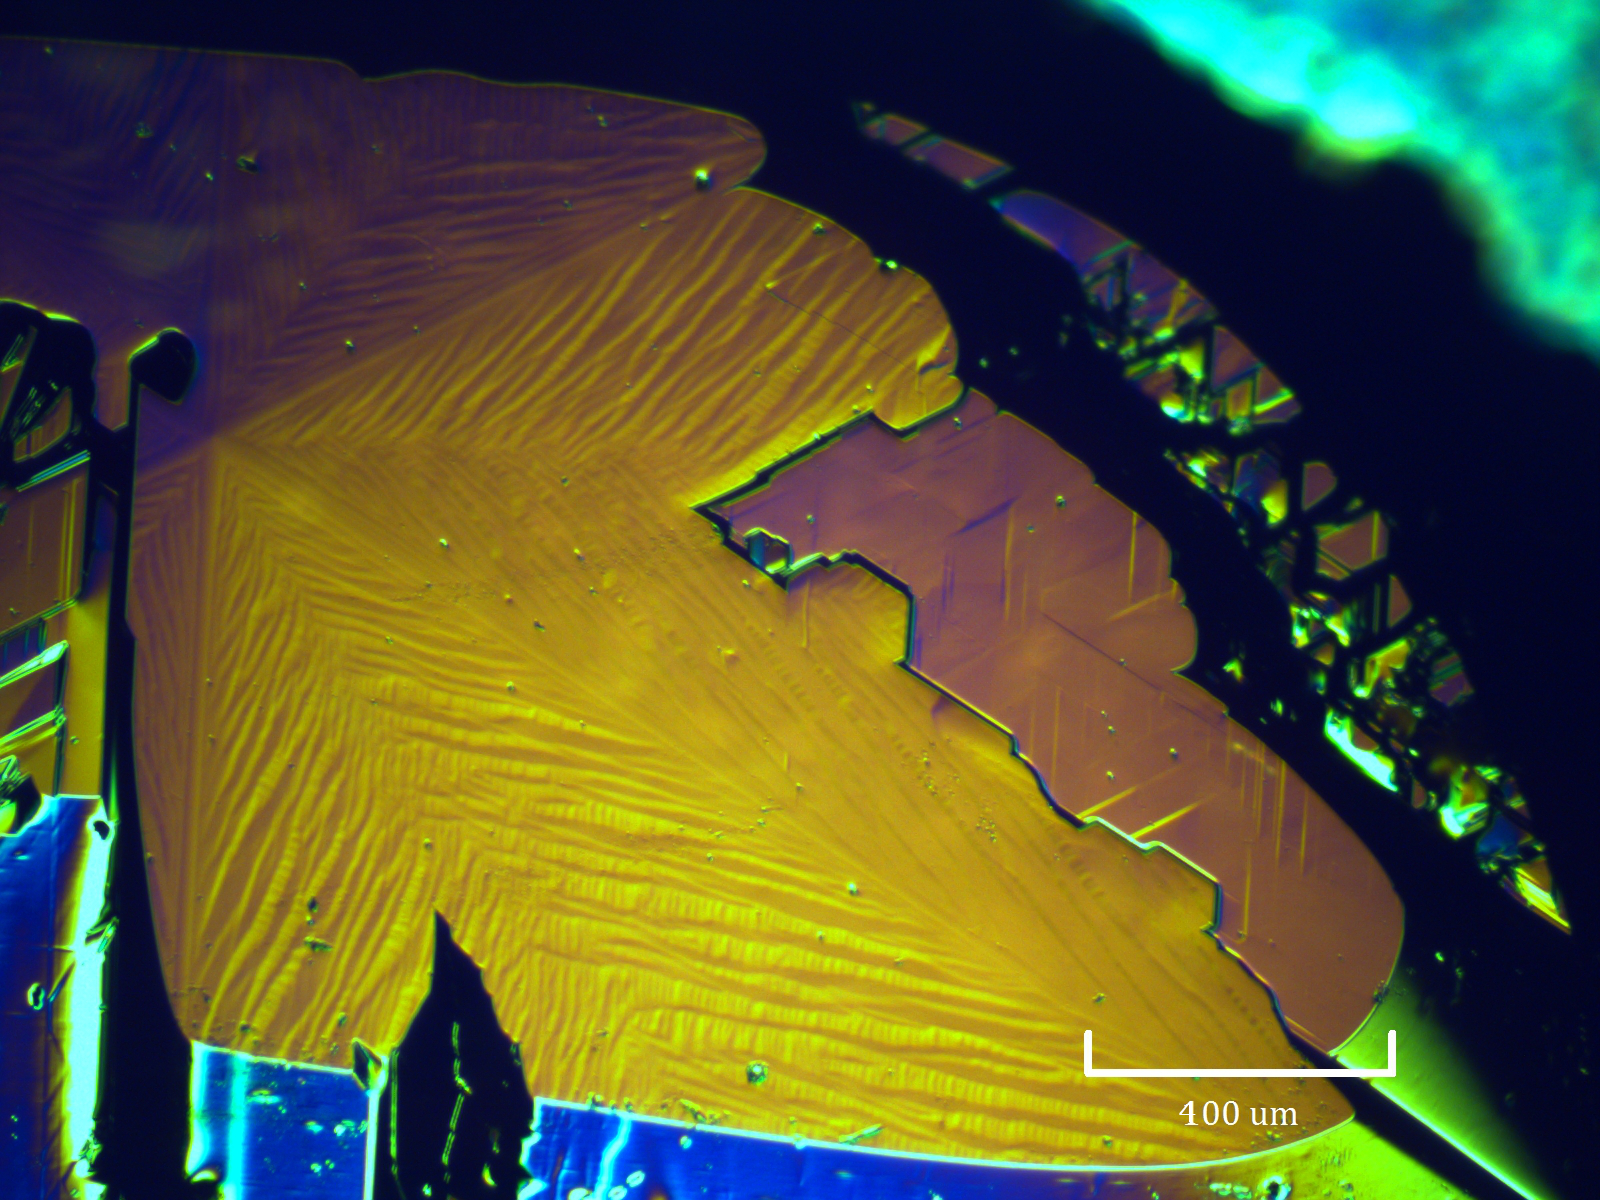
\includegraphics[scale=0.1]{C_seed1.jpg}
  \captionof{figure}{Reflection mode micrograph of the facet of C-face seed S5.}
  \label{fig:carbon_seed1}
\end{minipage}%
\begin{minipage}{.5\textwidth}
  \centering
  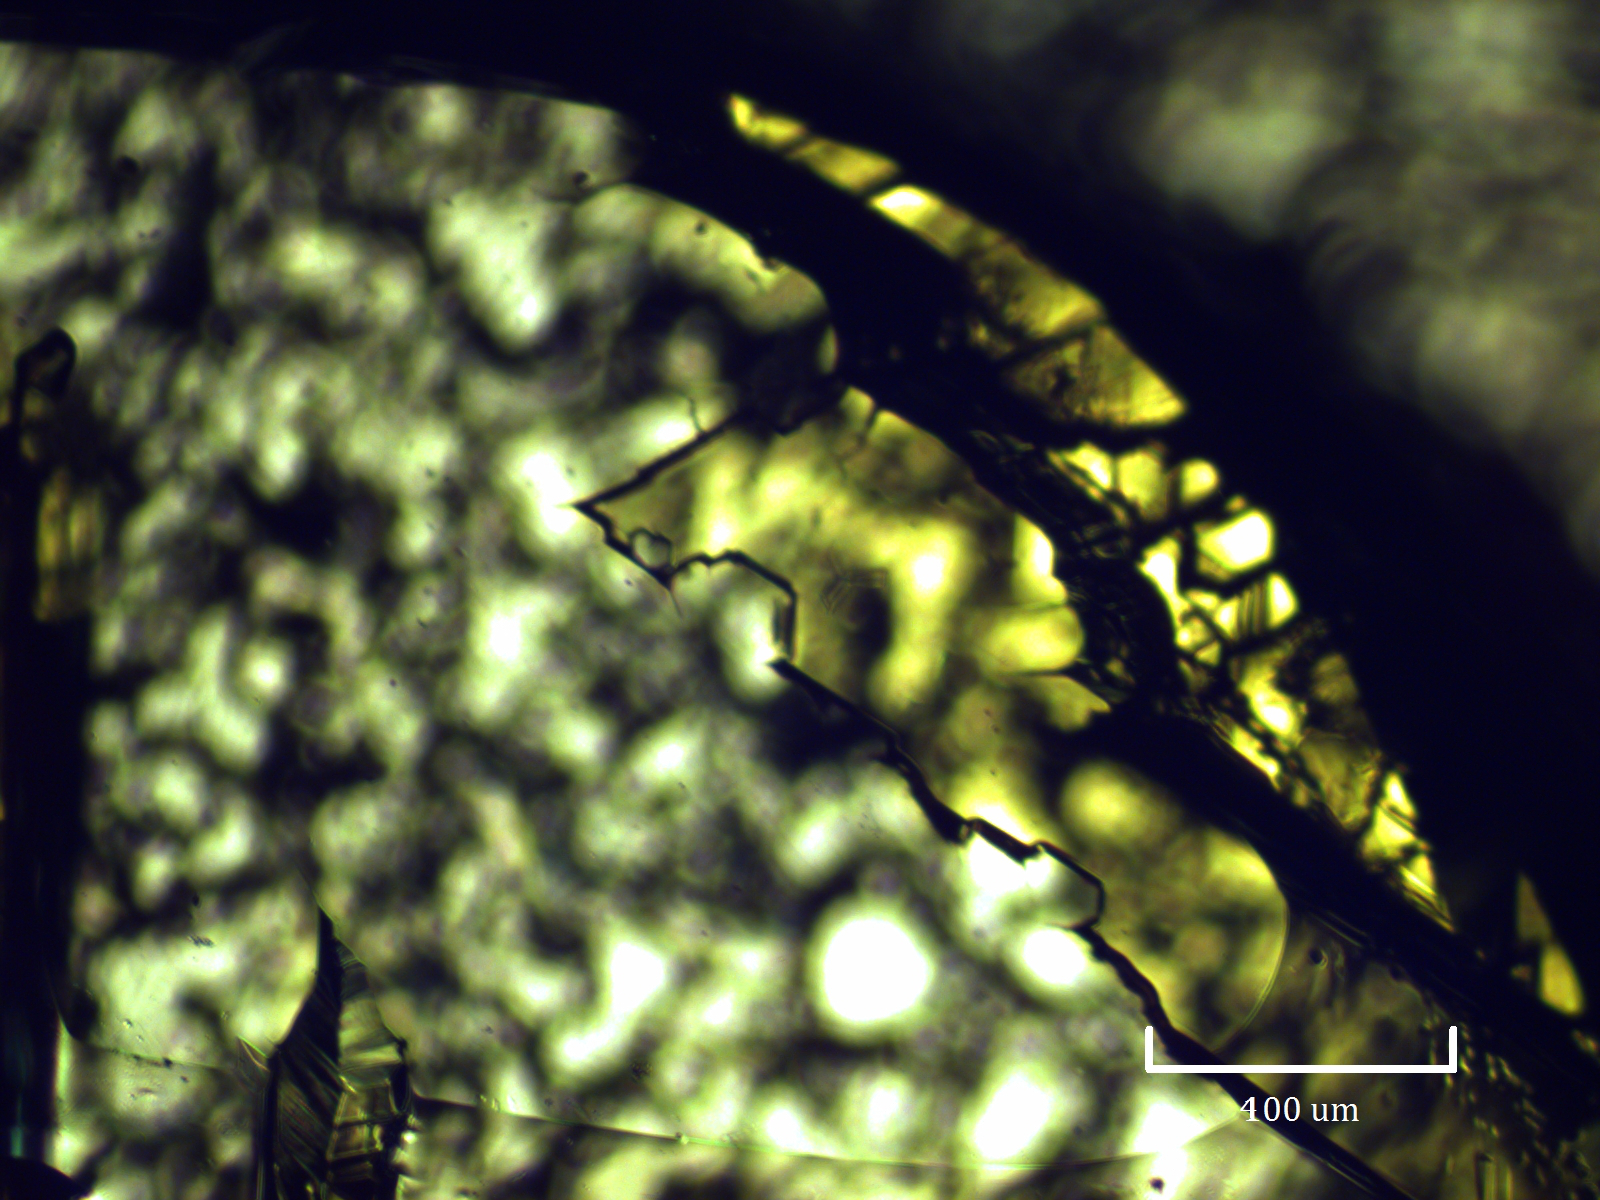
\includegraphics[scale=0.1]{C_seed2.jpg}
  \captionof{figure}{Nomarski transmission mode micrograph of the facet of C-face seed S5.}
  \label{fig:carbon_seed2}
\end{minipage}
\end{figure}

Figure \ref{fig:silicon_seed} shows a reflection mode silicon face grown seed. On this sample the whole facet is covered with the 3C-SiC polytype. This micrograph is representative of the Si-face grown seeds, most of which had complete facet coverage. 

\begin{figure}[H]
\begin{center}
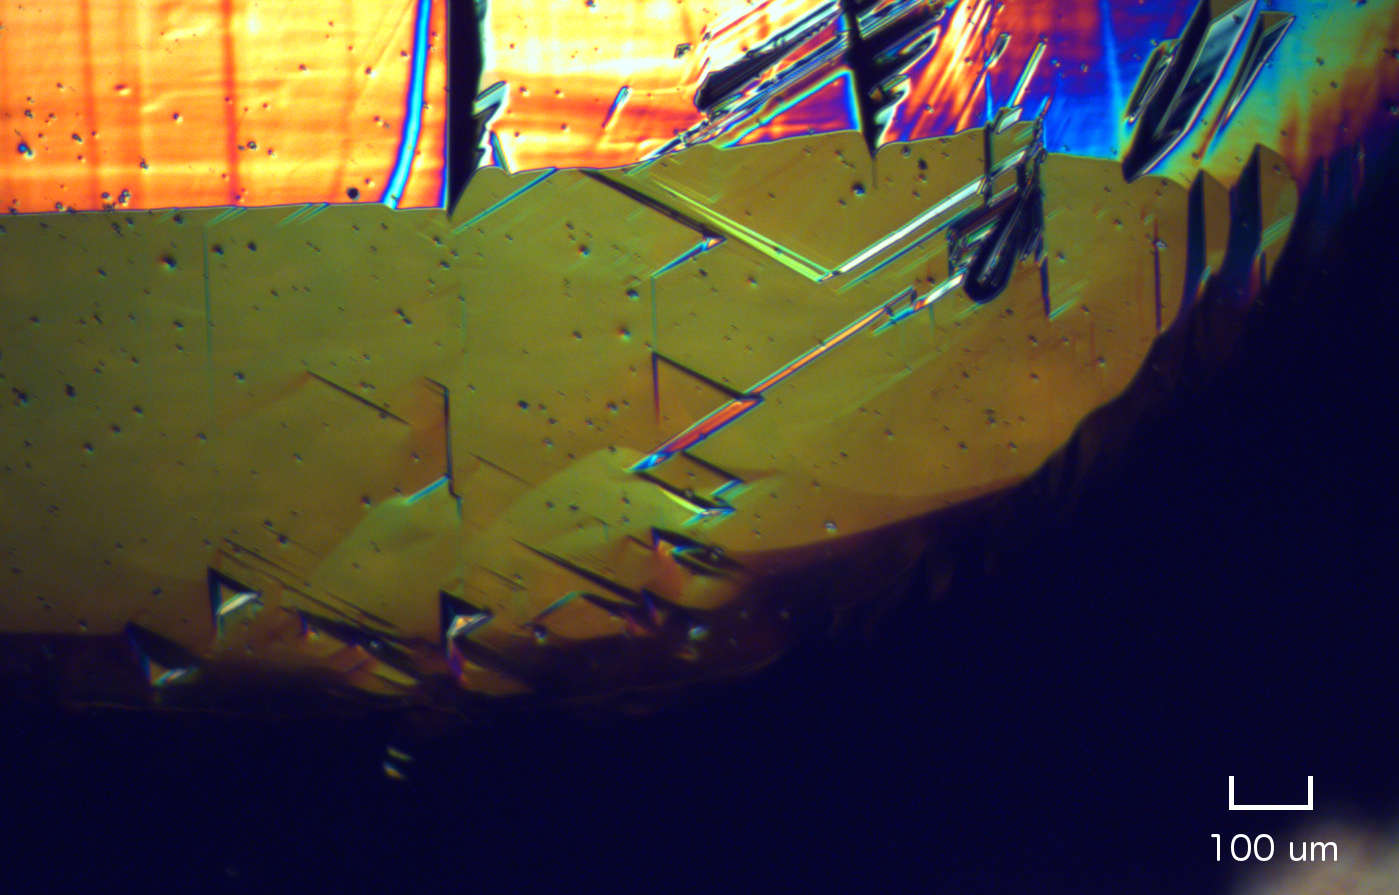
\includegraphics[scale=0.15]{undoped_Si_face.jpg}
\caption{Reflection mode micrograph of the facet of a Si-face seed.
\label{fig:silicon_seed}}
\end{center}
\end{figure}




\section{On B-doped samples}
\label{sec:results:doped}
This section shows the results of characterization of B-doped samples. Table \ref{tab:doped_samples} shows the growth conditions and sample thickness of the grown B-doped samples. The thickness is measured for the doped layer, excluding both the substrate and the undoped seed. The growth mode is the stacking order of the doped and undoped source materials in the crucible, as described in section \ref{sec:growth:fsgp:doping}. The \emph{Seed} column displays whether the sample was grown on a 3C-SiC seed or on a 4H-SiC 4$^\circ$ off-axis substrate. All substrates used for B-doped samples are Si-face, and the seeds are all grown on Si-face. 

\begin{table}[h]
\caption{Growth conditions of the doped samples are shown in this table. The growth mode describes which samples are grown using direct or indirect doping methods. These methods are described in section \ref{sec:growth:fsgp:doping}. The doping concentration is given for the source material.} 
\label{tab:doped_samples}
\begin{center}
\begin{tabular}{l c c c c c r}
  \hline                       
  \hline       
  \vspace{1mm}
   & \small{Temp. [$^\circ$C]} & \small{Time [h:min]} & \small{Thickness [$\mu$m]} & \small{Doping [cm$^{-3}$]} & Mode & Seed\\
    \hline
  D1 & X & X:XX & X & 10$^{18}$&Direct & Yes\\ %S1
  D2 & 1825 & 2:30 & 350 & 10$^{18}$&Direct & Yes\\ %S3
  D3 & 1825 & 3:00 & 360 & 10$^{18}$&Direct & Yes\\	%S2
  D4 & X & X:XX & 440 & 10$^{19}$&Direct & Yes\\ %S1
  D5 & 1825 & 2:30 & 320 & 10$^{19}$&Direct & Yes\\ %S2
  D6 & X & X:XX & X & 10$^{20}$&Direct & Yes\\%S1
  D7 & 1825 & 2:30 & 220 & 10$^{20}$&Direct & Yes\\%S2
  D8 & 1825 & 2:30 & 380 & 10$^{18}$&Indirect & Yes\\%S3
%  2 & XXX & X:XX & X & 10$^{20}$&Indirect\\%S2 %BG proper
  D9 & 1825 & 2:30 & 380 & 10$^{20}$&Indirect & No\\%S3
  
  \hline  
\end{tabular}
\end{center}
\end{table}


\begin{figure}[h]
\begin{center}
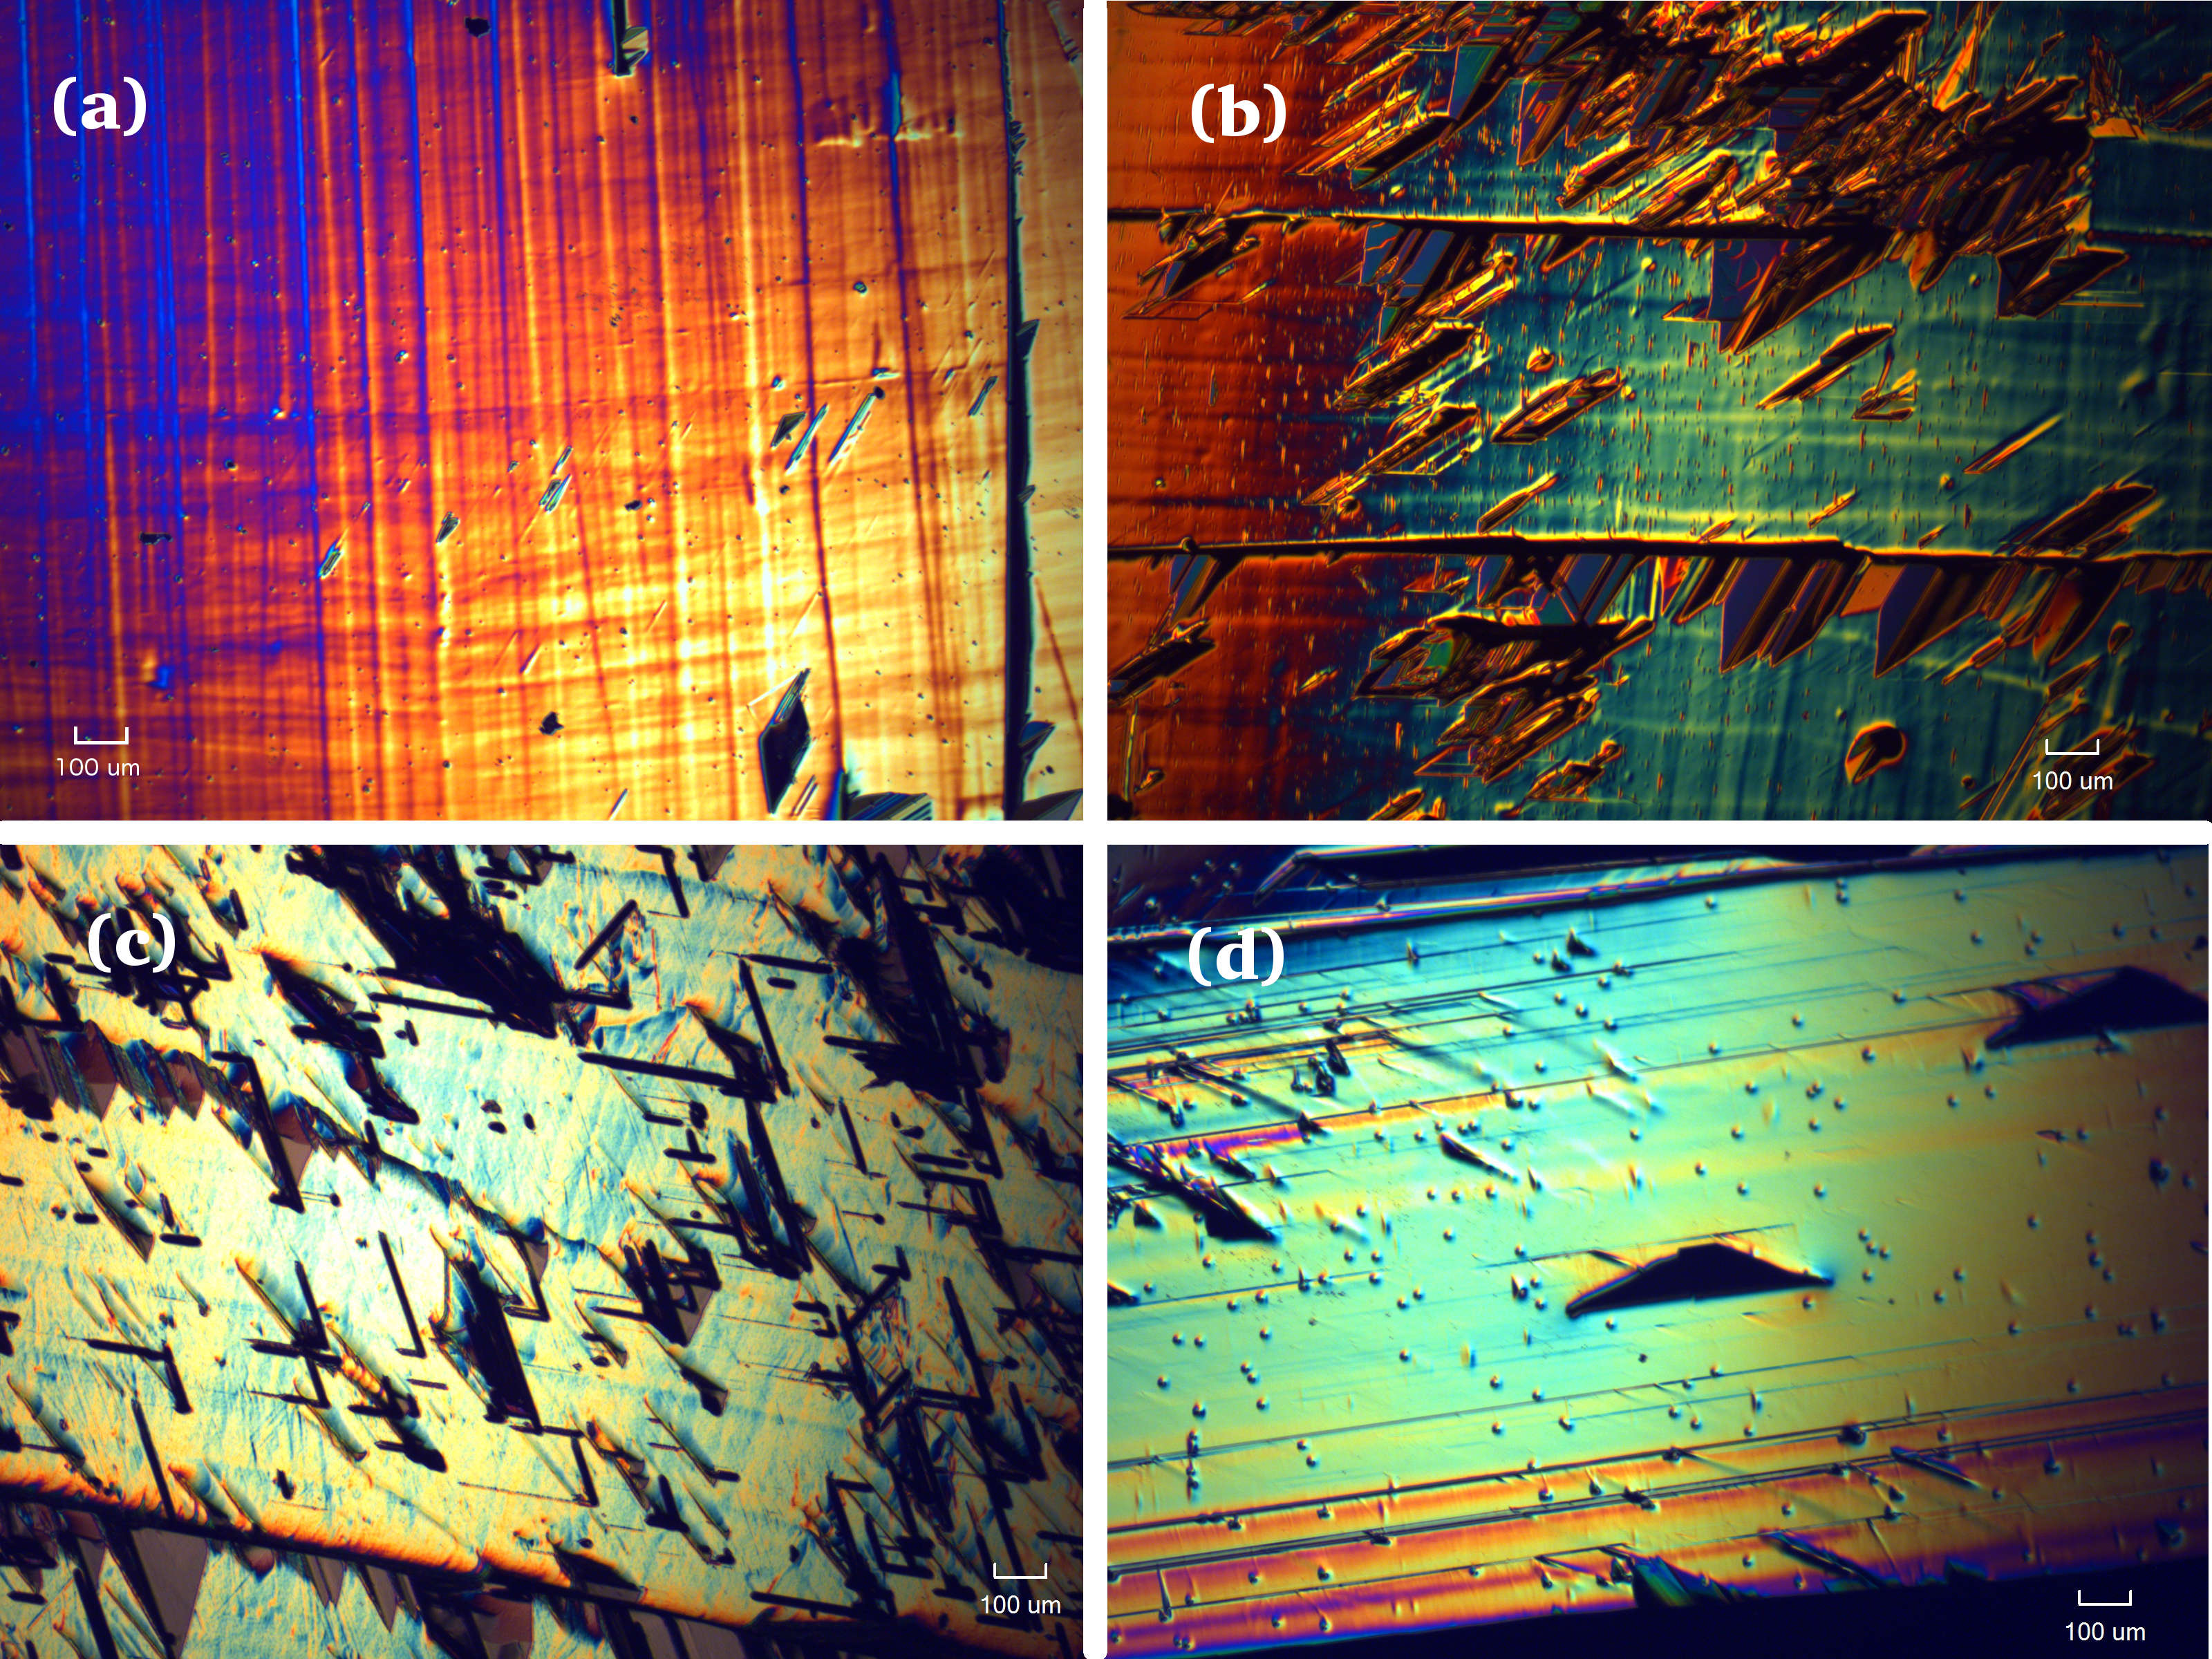
\includegraphics[scale=0.10]{doped_series_four.jpg}
\caption{Micrographs of an undoped sample (a), doped sample number D1 (b), doped sample number D4 (c) and doped sample number D6 (d).
\label{fig:B_doped_micrographs1}}
\end{center}
\end{figure}

Figure \ref{fig:B_doped_micrographs1} shows the surface morphology of an undoped sample (a), doped sample number D1 (b), doped sample number D4 (c) and doped sample number D6 (d). It is clearly seen that the undoped sample has a better crystal quality compared to (b) and (c), but (d) which is grown with a highly doped source shows good crystal quality. The micrographs are representative for the whole surface morphology of the samples. It should be noted that the samples (b)-(d)   are grown using a source material doped with dopant concentration of 10$^{18}$, 10$^{19}$ and 10$^{20}$ cm$^{-3}$ respectively.

Figure \ref{fig:B_doped_micrographs2} shows micrographs of samples D1 (a) and D8 (b). It should be noted that the two samples are grown with direct and indirect doping methods respectively. It can be seen that the sample surface quality is similar in the two samples. 

\begin{figure}[H]
\begin{center}
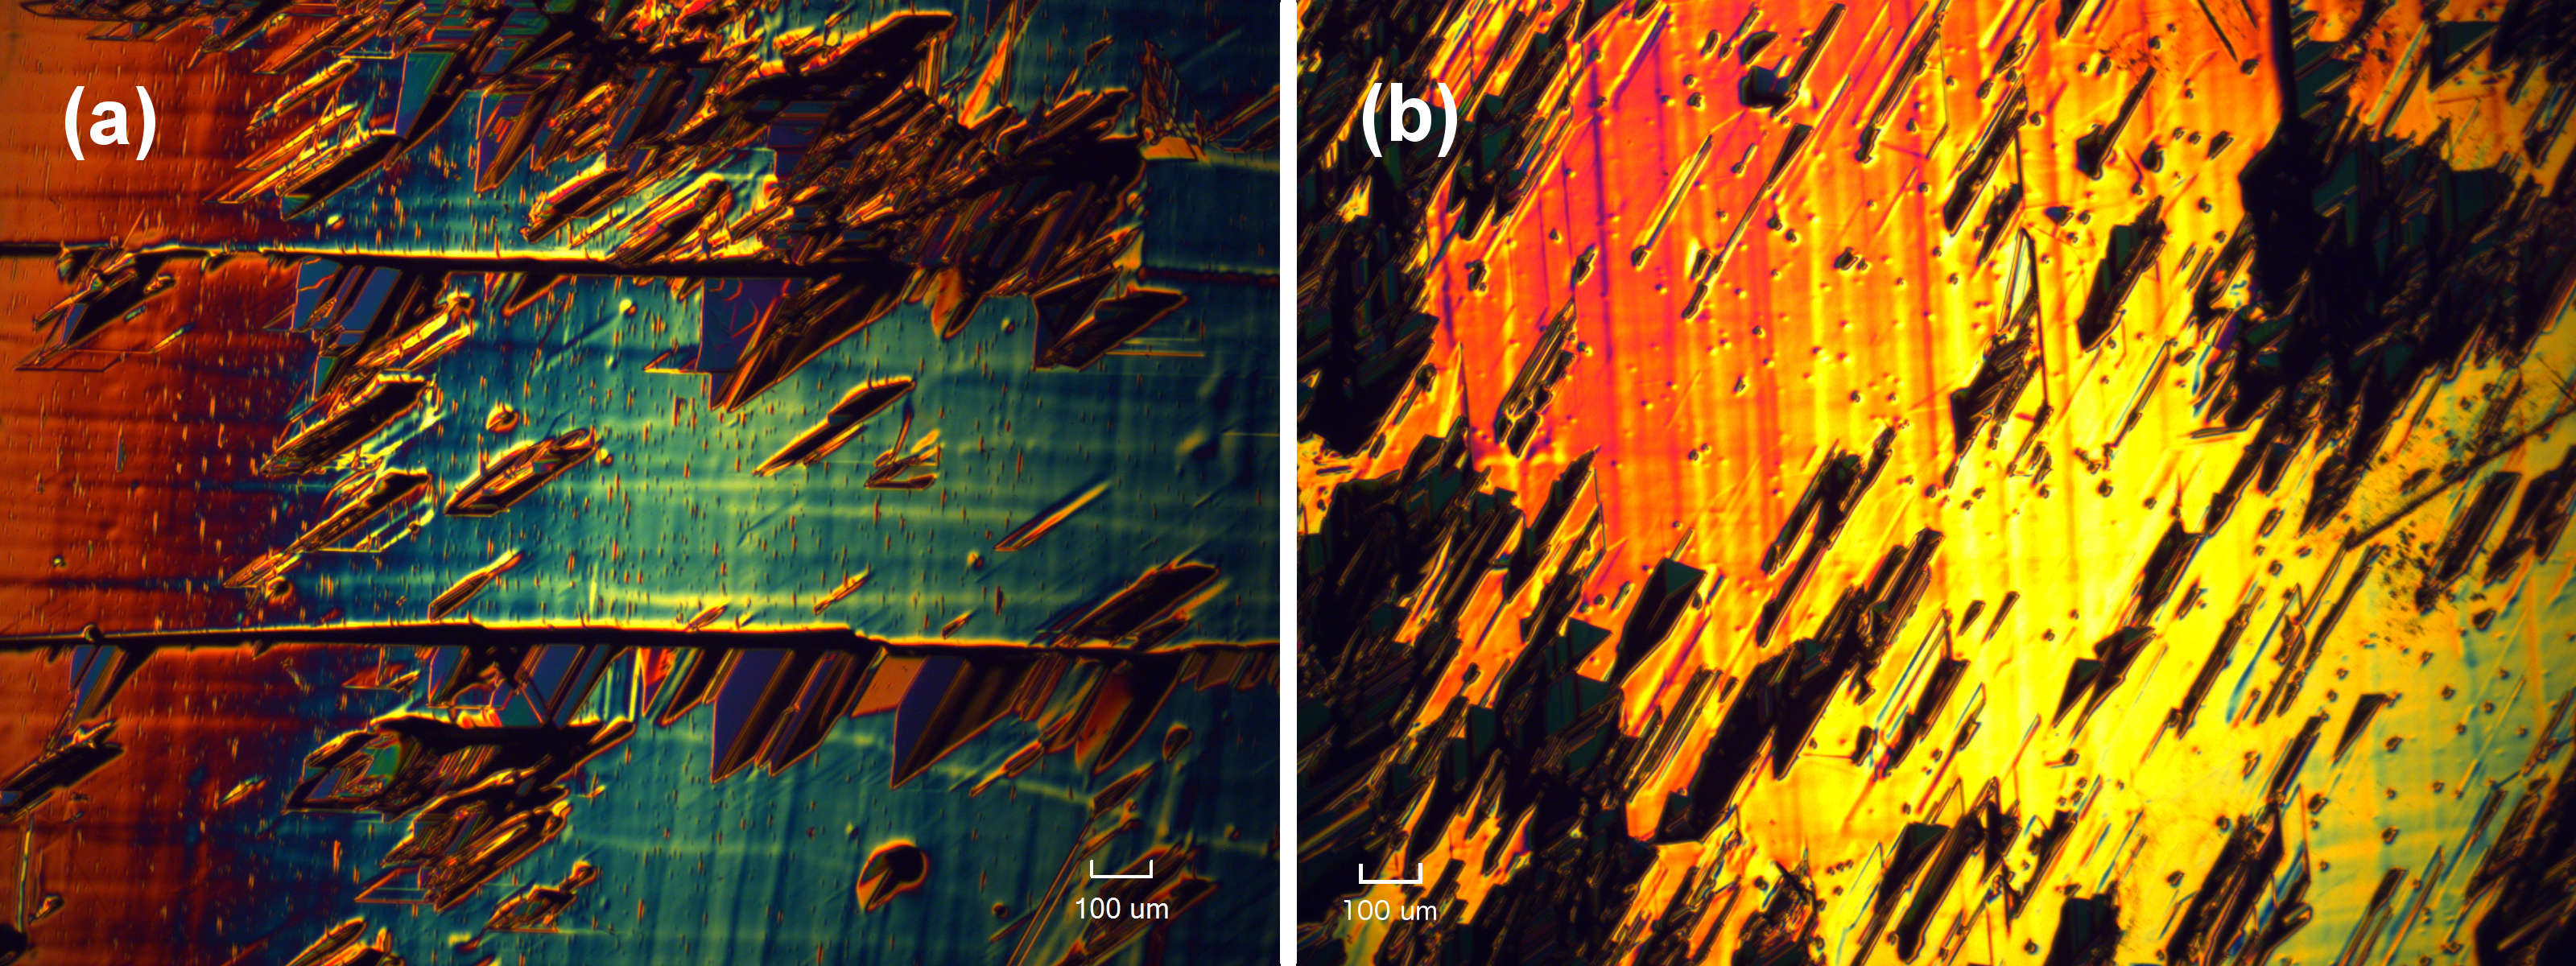
\includegraphics[scale=0.11]{direct_indirect_e18.jpg}
\caption{Micrographs of samples D1 (a) and D8 (b). 
\label{fig:B_doped_micrographs2}}
\end{center}
\end{figure}


Figure \ref{fig:BGe20_micrograph} shows reflection mode micrographs of samples D6 (a) and D9 (b). These samples are grown with direct and indirect growth methods respectively. Both samples show comparable surface morphology. In (c) a transmission mode micrograph of D9 is shown. It can be seen that there are two different polytypes in the sample. The brighter area in the center is a foreign polytype inclusion. 

\begin{figure}[h]
\begin{center}
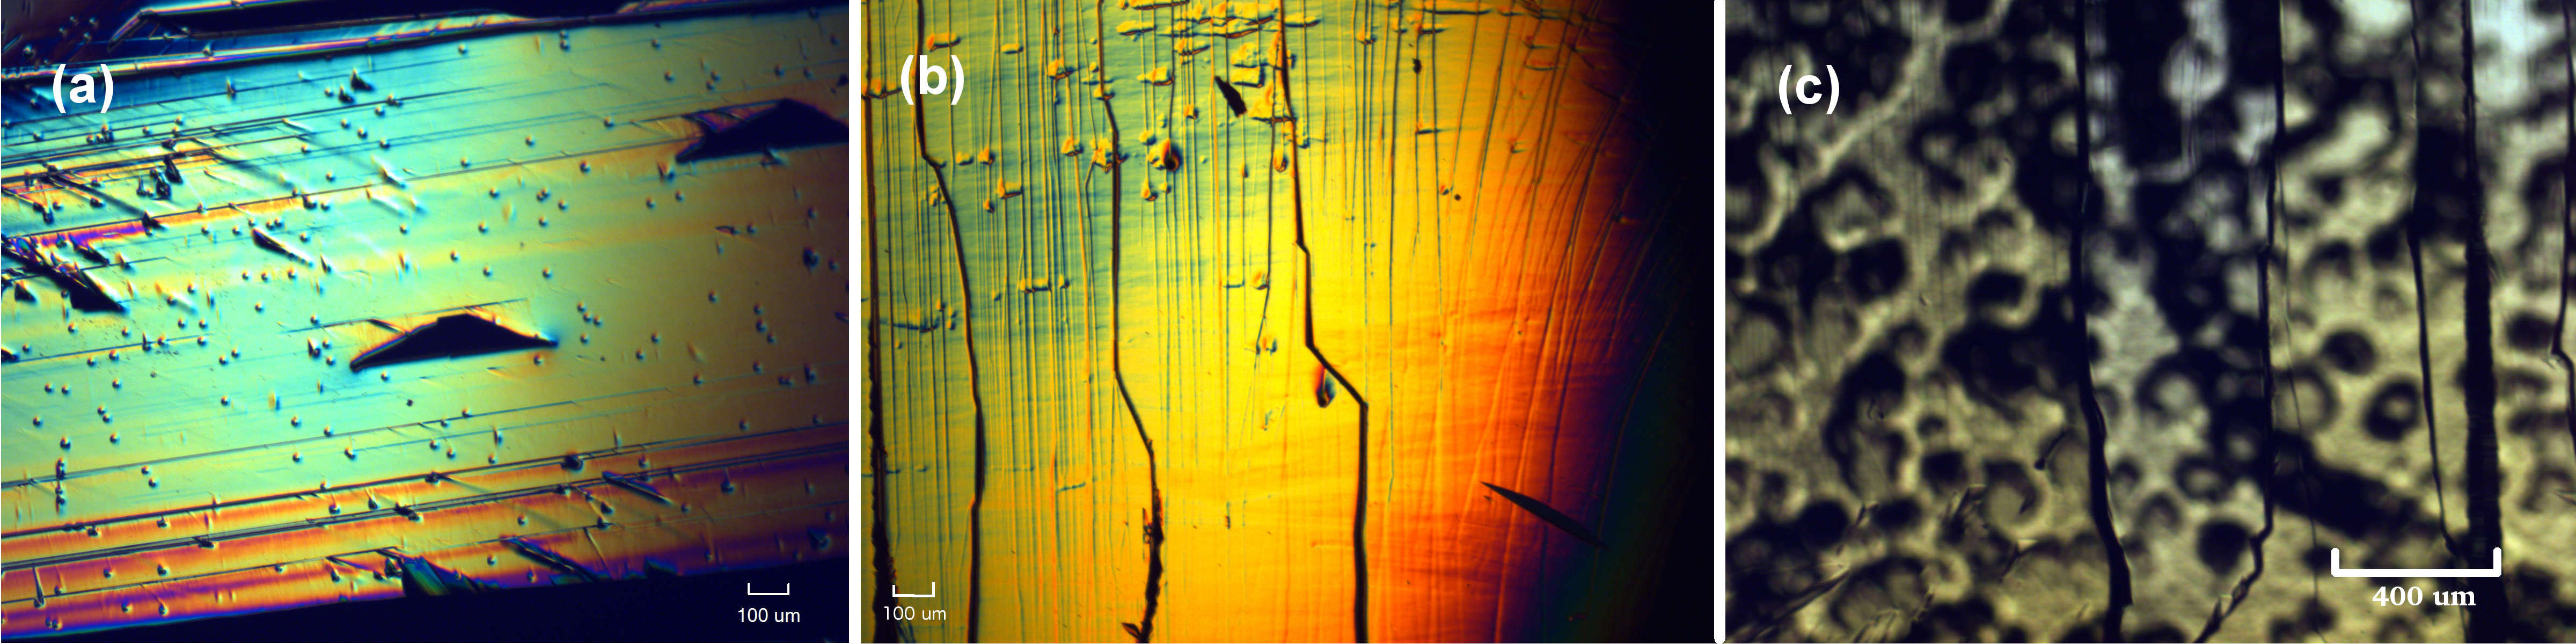
\includegraphics[scale=0.07]{direct_indirect_e20.jpg}
\caption{Reflection micrographs of samples D6 (a) and D9 (b), and transmission micrograph of D9 (c). 
\label{fig:BGe20_micrograph}}
\end{center}
\end{figure}

Absorption measurements were done on directly doped samples with different source doping concentrations, samples D1 and D5. The results of these measurements are shown in figure \ref{fig:abs1}, together with a reference spectrum from an undoped sample (dotted line). In both samples we see the band edge absorption at around 500 nm. A second feature in the doped sample spectra is the peak at around 700 nm, corresponding to the transition between the boron level and CB. This cannot be seen in the undoped sample. The doped samples show no evidence for a VB to boron transition, which should be seen at around 1800 nm, as described in chapter \ref{sec:doping_in_3C}. Absorption was also measured for doped samples D6 and D7, but neither the band edge nor the boron related peaks were seen in these highly doped samples. 

\begin{figure}[h]
\begin{center}
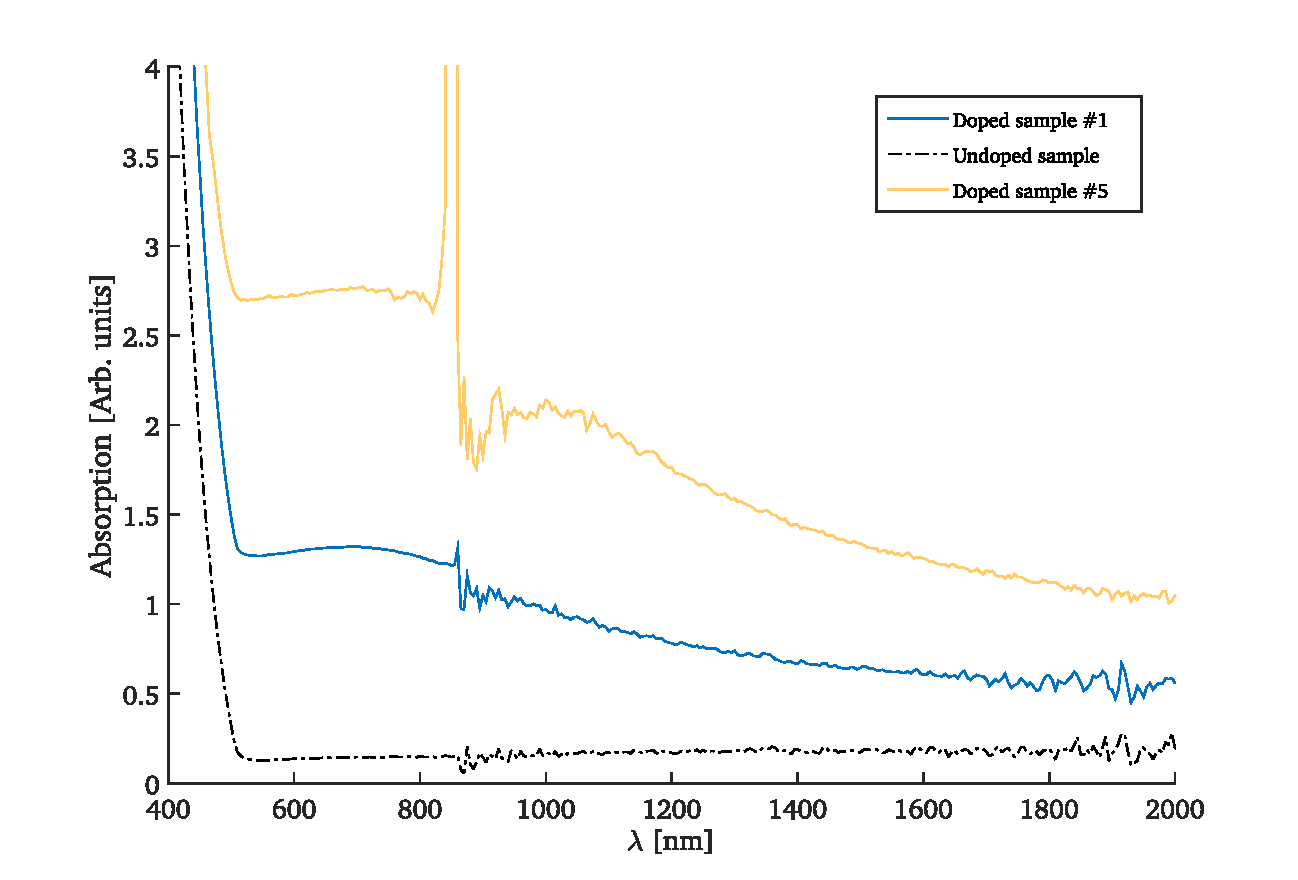
\includegraphics[scale=0.5]{absorption1.pdf}
\caption{Absorption spectrum of undoped sample (dotted line), doped sample D5 (bright yellow line) and doped sample D1 (dark blue line). 
\label{fig:abs1}}
\end{center}
\end{figure}

\begin{figure}[h]
\begin{center}
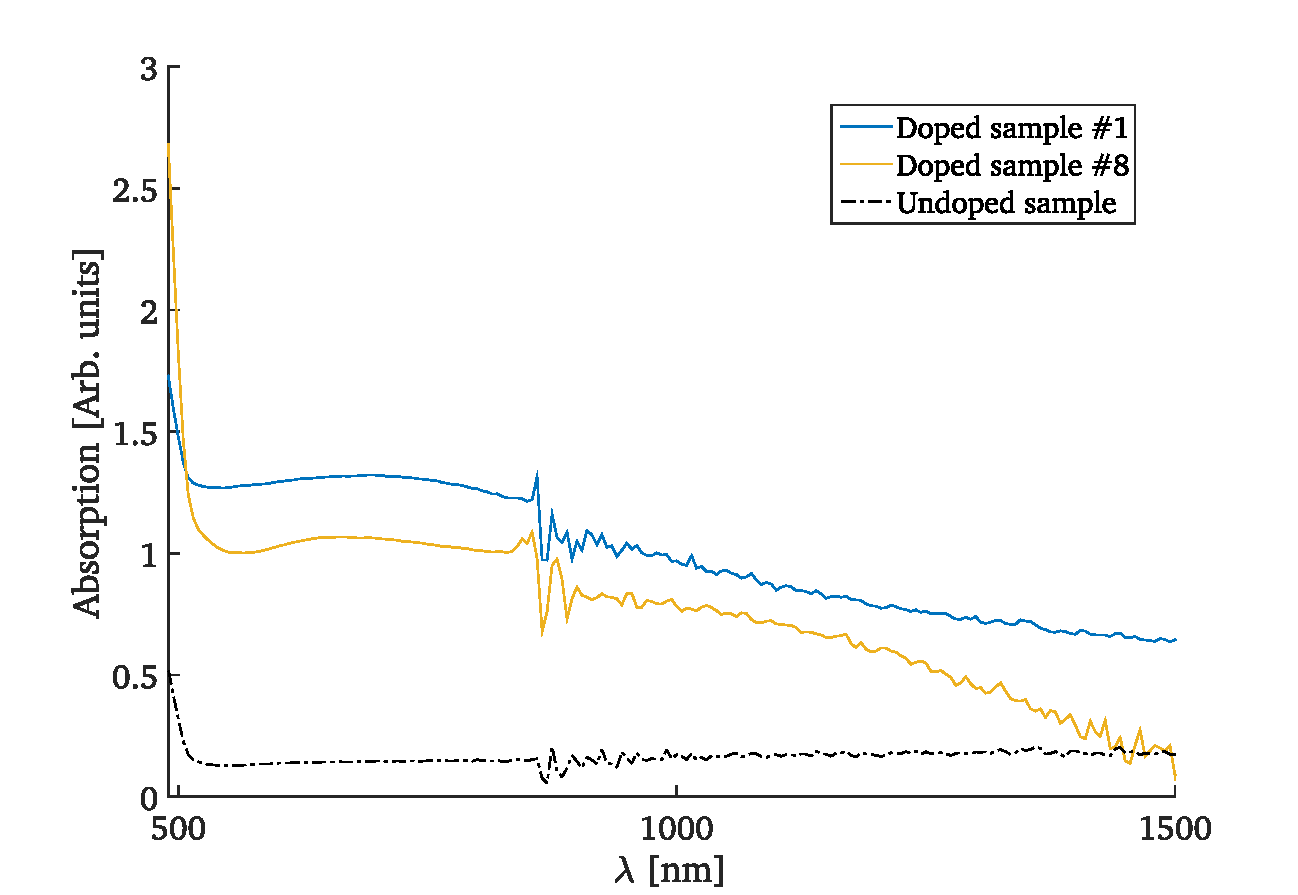
\includegraphics[scale=0.5]{absorption2.pdf}
\caption{Absorption spectrum of doped samples D8 (bright yellow line) and D1 (dark blue line), shown together with an undoped sample (dotted line). 
\label{fig:abs2}}
\end{center}
\end{figure}

Figure \ref{fig:abs2} shows the result of absorption measurements on samples D1 and D8, together with an undoped sample. It should be noted that D8 is an indirectly doped sample. It can be seen that both the doped sample spectra show the same trend. The graphs increase up to a point near the 700 nm B-N transition energy, where they level out. This is not visible in the undoped sample. It can further be seen that sample D8 has its B-N maximum at a slightly shorter wavelength compared to sample D1, which is attributed to the fact that measurements were done on D8 before polishing. The peak shift is in fact a substrate artifact. Absorption measurements were also done on sample D9, which did not show the B-CB peak. 



LTPL-measurements were done on boron doped samples and on an undoped seed. Figure \ref{fig:pl_spectrum1} shows the resulting spectrum of the undoped seed. Five peaks can clearly be seen in the spectrum, labeled as ZPL and phonon replicas. It should be noted that the ZPL is significantly smaller than the phonon replicas. It can further be seen that several smaller peaks appear on the low energy side of the phonon replicas. These lines originate from exciton complexes.  

\begin{figure}[h]
\begin{center}
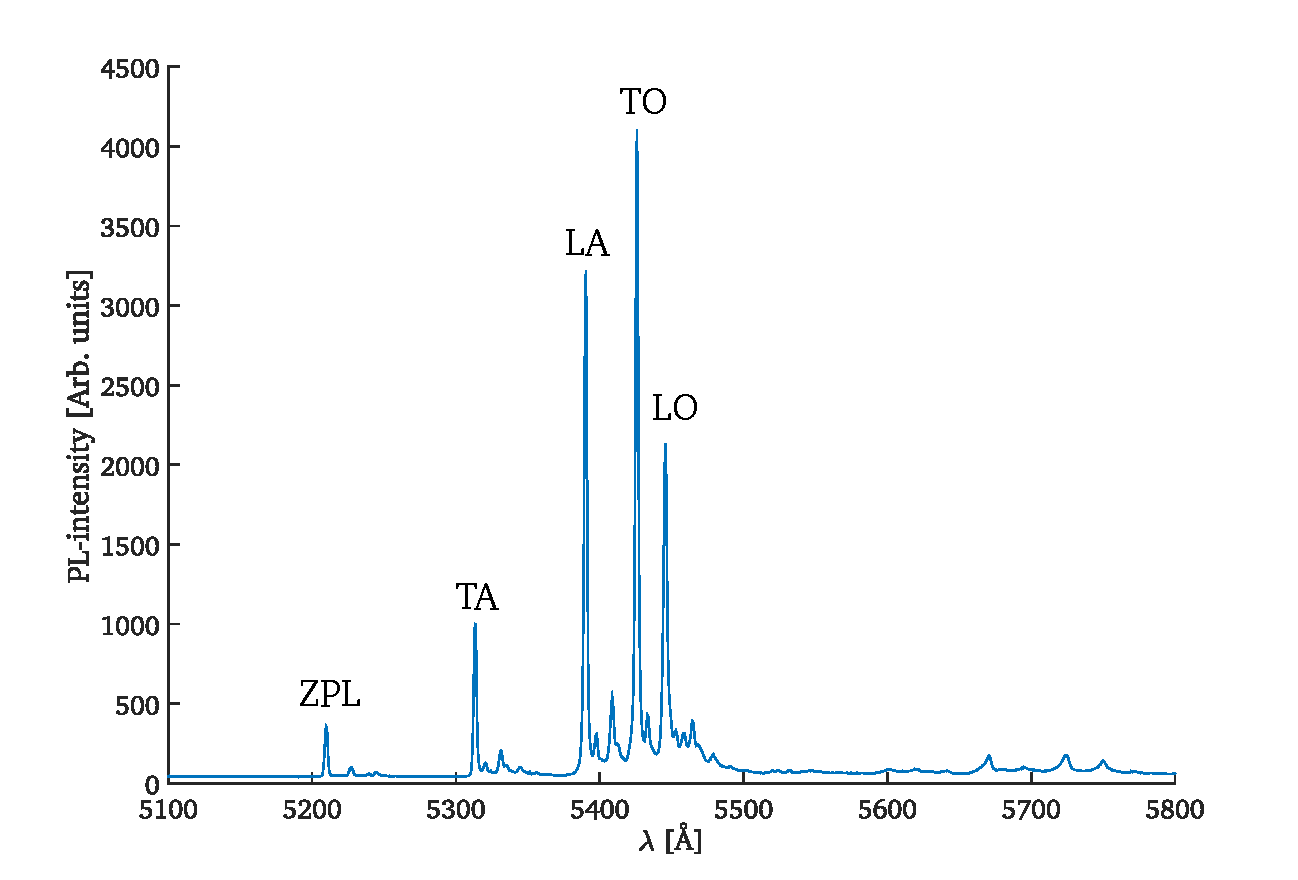
\includegraphics[scale=0.5]{PL_plot1.pdf}
\caption{LTPL spectrum of an undoped seed. The five main peaks are labeled as ZPL and phonon replicas. 
\label{fig:pl_spectrum1}}
\end{center}
\end{figure}

As described in chapter \ref{sec:pl}, the strain in a crystal can be estimated by the fraction between the LA and TO lines. From figure \ref{fig:pl_spectrum1} this is found to be 
\[I_\mathrm{LA}/I_\mathrm{TO} = 0.783.\]
From the TA-line FWHM, the donor concentration can be found. The FWHM is found to be $\Gamma_{TA} = 1.094$ meV, giving a nitrogen concentration of 
\[[N] \approx 10^{16} \, \mathrm{cm^{-3}}.\]
This value was obtained by using the same parameters as proposed by Camassel et al. \cite{Camassel2006}. 

Doped samples D1, D4 and D6 were measured using LTPL. Not one of these samples show any luminescence. Sample D9 did show luminescence from the hexagonal inclusions, but not from the cubic area. The spectrum is shown in figure \ref{fig:pl_spectrum2}. 

<Figure>.



































\label{sec:results}

%-*- mode: LaTeX; -*-

\chapter{Discussion}
\label{sec:discussion}
This chapter discusses the results presented in chapter \ref{sec:results}. The chapter is divided into two parts, one part discusses the results of seed growth and the other part discusses the results from characterization of the B-doped samples. 

\section{Seed growth}
As shown in section \ref{sec:results:seeds}, the carbon face grown seeds did not have complete coverage of cubic SiC on the terrace, yet the silicon face grown seeds could reproducibly be grown with complete cubic coverage. As seen in figure \ref{fig:supersaturation}, 2D growth is promoted by high supersaturation. A possible explanation of the results is that the supersaturation for the C-face growth was too low. The examined temperatures, as shown in table \ref{tab:seeds}  range from 1825 to 1925 $^\circ$C, which is a large portion of the parameter space in which the 3C-SiC polytype is stable. Changing the temperature much more during growth is unlikely to result in better 3C-coverage, since this will likely be outside the region where 3C-SiC can be formed in a stable manner. Because of this, the supersaturation will not be able to be changed much more by altering the temperature. 

From table \ref{tab:seeds} it can be seen that the percentage of the terrace covered by 3C-SiC does not show any trend with regards to temperature. The growth time has been adjusted to get similar sample thickness for all samples. In this way it was possible to vary only the supersaturation between samples. This indicates that for the used growth setup it is not possible to change the supersaturation enough to get complete 3C-SiC coverage of the terrace. However, the pressure conditions for growth have not been explored in this work, and that it may be possible to alter the ambient pressure to get more cubic coverage. 

A possible explanation of the difference in 3C-SiC coverage on silicon and carbon face substrates is the spiral growth character. On Si-face the spirals take the form of proper spirals, with steps expanding from the spiral arms. The C-face spiral takes the form of straight lines extending radially from the center, as seen in figure \ref{fig:carbon_seed1}. The 3C-SiC polytype nucleates on top of the heteroepitaxially grown spirals and grows over the spiral steps. The spiral shape can then be expected to influence how the 3C-SiC is grown. The silicon face spiral may be advantageous for cubic growth, while the carbon face spiral may not be. Another possible explanation is that there may be some difference between how the Si- and C-surfaces look for off-axis cut samples. There may be a difference in the number and density of the steps, which in turn will influence the terrace growth. To get a proper understanding of this, electron microscopy would have to be done on the substrate surface and the terrace after initial nucleation. In this way a proper understanding of the growth mechanisms governing C- and Si-face growth would be possible. This is beyond the scope of this work, but could be included in future work. 

The silicon and carbon faces have different surface energies which will influence how material grows on it. Stein et al. have shown that SiC growth on 4H-SiC and 6H-SiC substrates will result in different polytypes grown depending on the face rather than the substrate polytype. This they attributed to the different surface energies of the different faces \cite{Stein1992}. This may also be a factor in the problem of growing 3C-SiC on the carbon face. From the micrographs of the carbon face seeds it can be seen that cubic growth always occurs at the edge of the facet, i.e. near the graphite spacer. This is consistent with the hypothesis that the surface energy gives rise to the results since the edge is expected to have a different surface energy compared to somewhere towards the center of the sample. 

%\begin{itemize}
%\item Possible explanation is that the supersaturation is too low (see graph). Supersaturation varies with temperature, we should see a trend when varying temperature. We do not. 
%\item Cannot vary temperature much more, since 3C is only stable in small temperature window. 
%\item Spiral shape is different, maybe this shape is not good for 2D-growth. 
%\item C and Si has different surface energies, which will influence growth. Maybe the C conditions are not compatible with the 3C-growth. 
%\item The surface energy alternative explains why we always see 3C at the edge, never in the center.  
%\end{itemize}

\section{B-doped samples}
From figure \ref{fig:B_doped_micrographs1} it can clearly be seen that B-doping deteriorates the crystal quality. All doped samples have a larger number of defects compared to the nominally undoped sample. For samples D1 and D4 the number of defects increase with increasing source doping. This is to be expected since the boron atoms have a different radius compared to both the silicon and carbon atoms they replace. This size difference will induce strain in the sample and in turn induce defects. From the same figure we can see that sample D6, which was grown with the source material with the highest doping concentration, has a smoother surface compared to the two other doped samples characterized in this thesis. This does not follow the trend. In figure \ref{fig:BGe20_micrograph} (b) can be seen that sample D9, grown from the same source material as D6, shows similarly good surface quality. In contrast sample D8, again grown from the same source material, has a much poorer surface. From the absorption measurements on these samples it can be inferred that these materials do not in fact have very good quality. As described in chapter \ref{sec:results}, samples D8 and D9 do not show any B-CB absorption peak, and D6 does not show the band edge absorption. One possible explanation of this is that the source material does not in fact have the high doping concentration it is thought to have. This hypothesis is contradicted by the result of absorption measurement on D6. If the samples would be only lightly doped, then the band edge absorption would still be visible. Another possible explanation is that even though the surface shows a low density of defects, the sample may be of poor crystal quality. This would explain why sample D6 does not show any band edge absorption. Further characterization of the crystal quality of these samples would give more insight to why the surfaces seem smooth but the absorption measurements yield poor results. 

Figure \ref{fig:B_doped_micrographs2} shows the difference in surface morphology of doped samples D1 and D8, which have been grown using the direct and indirect growth methods, respectively. The fact that they both show similar numbers of surface defects could indicate that both samples have been doped with comparable concentrations of boron. As shown earlier a higher concentration of boron will induce more defects on the surface. Figure \ref{fig:abs} (b) gives a further indication that this hypothesis is valid. This figure indicates that the two samples give similar absorption spectra. Most importantly both spectra show the B-CB peak at around 700 nm. From this it can be suggested that the indirect doping method introduced in this work is able to introduce impurities in a grown sample. The density of introduced impurities is from the results thought to be similar, but methods better suited to give impurity concentrations should be used to validate this finding. 

The doped samples D1-D5 and D8 all show band edge absorption and the B-CB absorption peak, but none of the samples shows the VB-B peak, which should be present at around 1700 nm. A possible explanation for this would be that the B-level is near or below the Fermi level, so that the occupancy of the level is too high to show much absorption. The Fermi level can be computed if the doping concentrations are known. It can be assumed that the nitrogen doping concentration is the same in doped samples as in unintentionally doped samples, i.e. the donor concentration is $N_D \approx 10^{16}$ cm$^{-3}$. Assuming that the B-doped samples are of p-type, i.e. $p>>n$, the neutrality condition is
\begin{equation}
\label{eq:neutrality1}
p = N_A^- - N_D^+.
\end{equation}
Since the nitrogen energy level is shallow, it can be assumed that at room temperature all donor atoms are ionized. This gives that $N_D^+ =N_D$. Under the Boltzmann approximation the hole density is
\begin{equation}
\label{eq:p}
p \approx N_Ve^{-E_F/kT},
\end{equation}
were $N_V$ is the valence band density of states, and is given by
\begin{equation}
\label{eq:nv}
N_V = 2\left(\frac{kTm_{d,h}}{2\pi \hbar^2}\right)^{3/2},
\end{equation}
where $m_{d,h}$ is the density of states hole mass. The number of ionized acceptor atoms is governed by the temperature and the distance between the Fermi level and the acceptor level, 
\begin{equation}
\label{eq:ionized}
N_A^- = \frac{N_A}{1+2e^{\frac{E_A-E_F}{kT}}}.
\end{equation}
From equations \ref{eq:p}-\ref{eq:ionized} the neutrality condition \ref{eq:neutrality1} can be rewritten as
\begin{equation}
\label{eq:neutrality2}
f(E_F) \equiv N_Ve^{-E_F/kT}+2N_Ve^{(E_A-2E_F)/kT}+2N_De^{(E_A-E_F)/kT} - N_A + N_D = 0,
\end{equation}
where the LHS is denoted $f(E_F)$. By using the values $E_A = 0.735$ meV, $m_{d,h} = 0.6m_0$ and $T = 300$ K, equation \ref{eq:neutrality2} gives the plots in figures \ref{fig:N_A} and \ref{fig:fermi}. In \ref{fig:N_A}, the graphs show the function $f(E_F)$ for different values of $N_A$, ranging from $10^{17}$ (light blue) to $10^{18}$ (dark blue) cm$^{-3}$. In figure \ref{fig:fermi} the Fermi level has been computed for concentrations ranging from $10^{16}$ to $10^{21}$ cm$^{-3}$. It can be seen that for concentration around 3$\times10^{17}$ cm$^{-3}$, the Fermi level is at 0.74 eV, which corresponds to the acceptor level. It is likely that the doping concentration in the sample is in the same order of magnitude, or smaller, as in the source material from which it was grown. From this it can be concluded that for doped samples grown with source impurity concentration of $10^{18}$ the Fermi level likely is near or above the acceptor level at room temperature. If the doping concentration of grown samples are significantly smaller than of the source material, then it is probable that also the samples grown from $10^{19}$ and $10^{20}$ cm$^{-3}$ sources have the Fermi level above the acceptor level. This may be the reason why the VB-B peak is not visible in the absorption spectra. 

\begin{figure}[h]
\centering
\begin{minipage}{.5\textwidth}
  \centering
  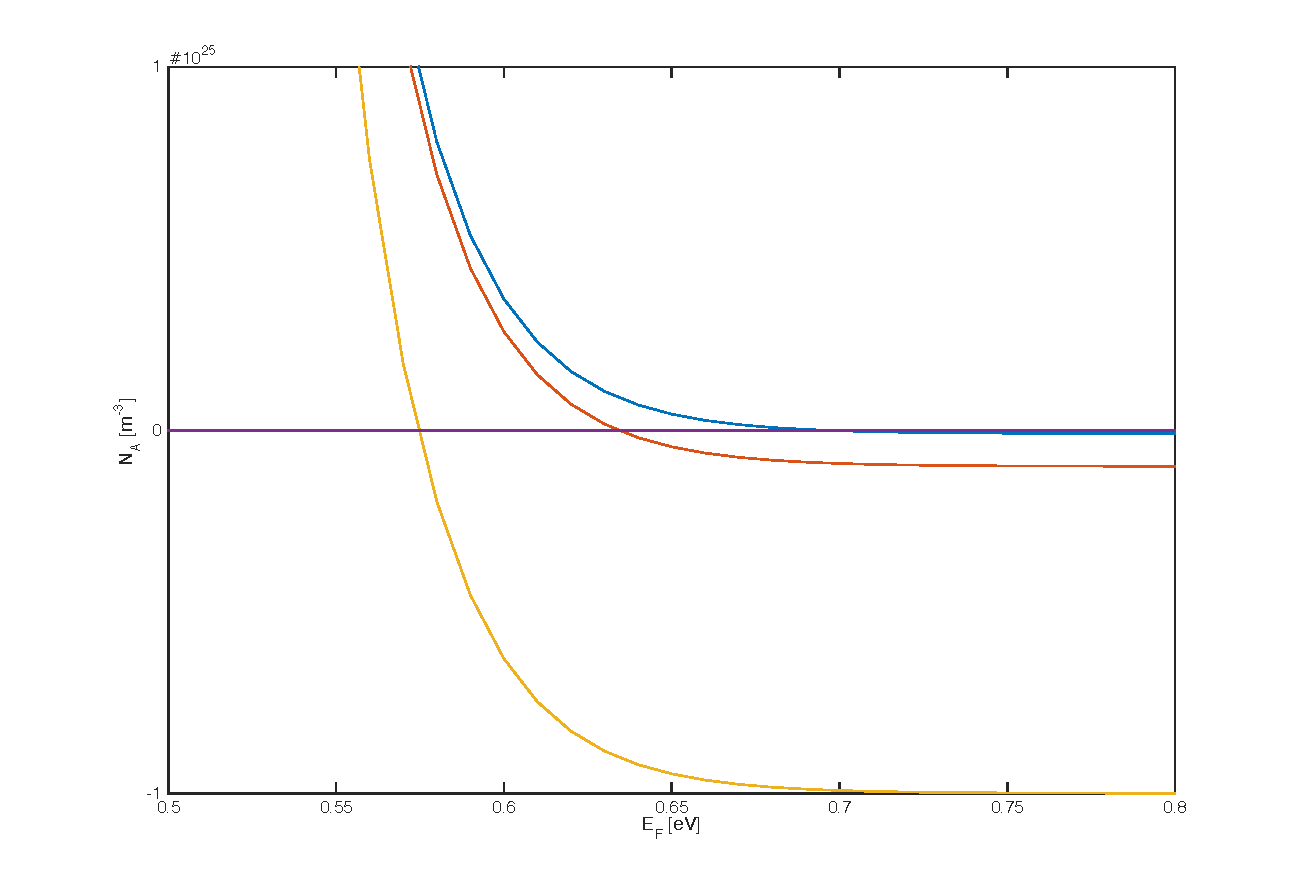
\includegraphics[scale=0.3]{N_A.pdf}
  \captionof{figure}{Computed values of LHS in equation \ref{eq:neutrality2}, plotted against the Fermi level. The three graphs show acceptor concentrations of $10^{17}$, $10^{18}$ and $10^{19}$ cm$^{-3}$. }
  \label{fig:N_A}
\end{minipage}%
\begin{minipage}{.5\textwidth}
  \centering
  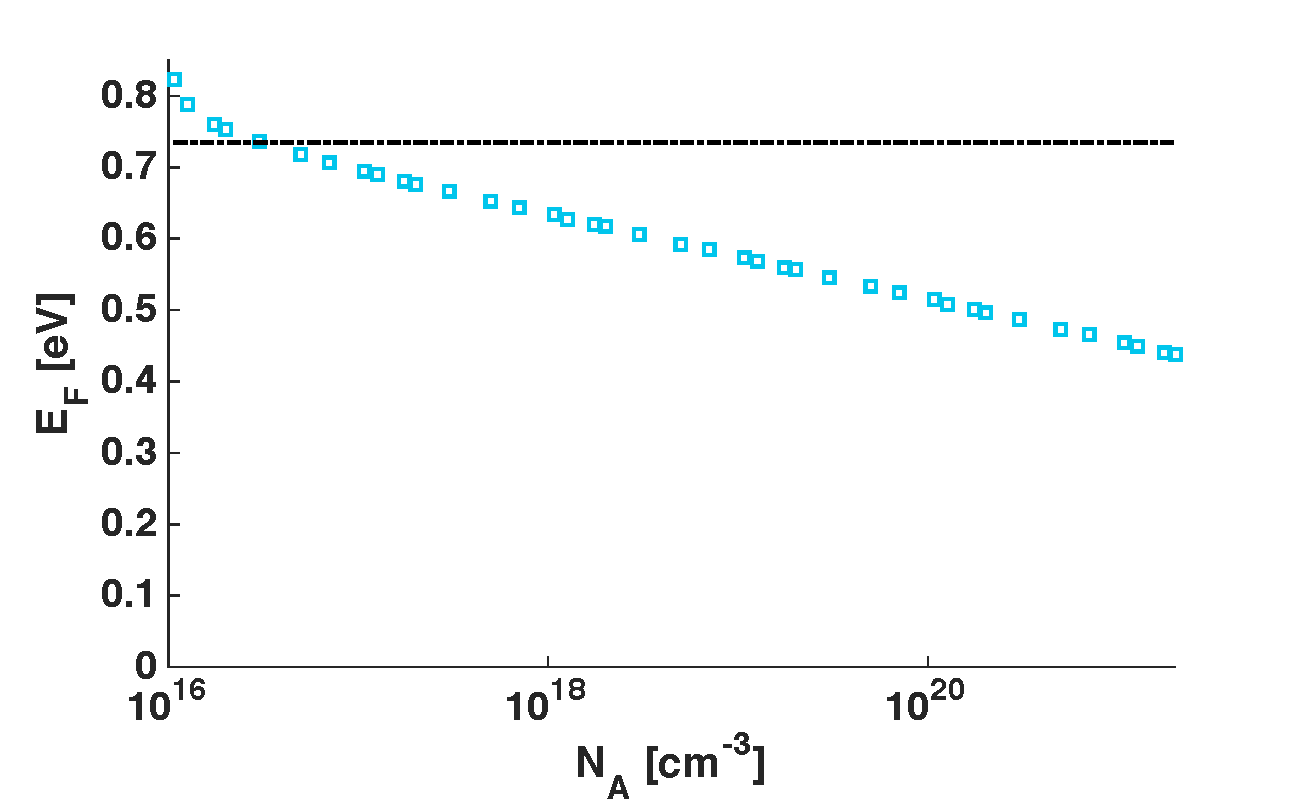
\includegraphics[scale=0.4]{Fermi.pdf}
  \captionof{figure}{Calculations of the Fermi level for different acceptor atom concentrations}
  \label{fig:fermi}
\end{minipage}
\end{figure}

Most of the B-doped samples showed no luminescence at all. One possible explanation for this is that the acceptor level is of non-radiative character. It is to be expected that boron, which is a deep level impurity, is of non-radiative character and recombines in a way which does not emit a photon, such as by the Shockley-Reed-Hall process \cite{Hall1952},\cite{Shockley1952}. There have, however, been reports of luminescence from B-doping levels in 3C-SiC, for example by Kubawara  et al. \cite{Company1976}. This means that the fact that the B-level may be to some extent non-radiative does not entirely explain why most of the doped samples measured show no luminescence. 

Another explanation of the PL-spectra from the doped samples is that the boron doped samples are not of sufficient crystal quality. As shown in figure \ref{fig:B_doped_micrographs1} the doped samples contain many defects. It may be that the many defects form non-radiative levels in the band gap and which compete with the boron level. This would explain why the results do not agree to those reported in literature. 

One sample (D9) did show luminescence at around 6000 Å which corresponds to an aluminium impurity level. As aluminium is a shallow acceptor, it will be able to capture carriers more easily compared to the deep levels created by boron. It is likely that more carriers are captured in the Al-level, which decreases the number of exciton recombinations from the B-level. This may be another explanation of why no boron related lines can be seen. There is luminescence from the hexagonal inclusions in this sample (inclusions are shown in figure \ref{fig:BGe20_micrograph} (c)). The luminescence is thought to originate from the B-CB transition. It is likely that both polytypes in the same sample have similar impurity concentrations for both B and Al. This is not consistent with the hypothesis that B-Al competition is responsible for the lack of B-lines in the 3C-SiC spectra. 














































\label{sec:discussion}

%-*- mode: LaTeX; -*-

\chapter{Conclusion}
Initially the idea was to investigate how C- and Si-face grown seeds differed in growth of B-doped samples. I was not able to reproducibly grow C-face seeds which were completely cubic. Investigating the seed growth I was able to show that however the temperature conditions were changed, 3C-SiC could not grow to cover the whole growth area on C-face substrates, while on the Si-face it was possible to reproducibly do so. The reason for this is not fully understood, but the reason may be the difference inherent in the surface of C-face and Si-face 4H-SiC, such as the surface energy of the surfaces. It may also be that the steps from the off-axis cut are different on C- and Si-faces, or contributed to the different form of the spirals. 

I have shown through optical microscopy that high B-doping leads to deteriorating surface quality of the sample. For most samples the surface quality worsened with increasing B-doping concentration of the source material. From optical microscopy and absorption measurements I have shown that it is possible to grow 3C-SiC material doped with boron using the sublimation growth technique described in this thesis. The absorption measurements indicate the boron to conduction band transition, but not the valence band to boron transition. The lack of the latter is thought to be due to the position of the Fermi level near or above the boron level in the band gap. 

I have shown using LTPL-spectroscopy that the boron levels in 3C-SiC grown in this work show no luminescence related to boron. The reason for this may be a combination of the deep level nature of the boron impurity with the poor crystal quality containing non-radiative defects. These PL-measurements further show inclusions of aluminium in the samples, which may form a competing relationship with the boron in carrier capture, further limiting the possibilities of luminescence. 
\label{sec:conclusion}

%-*- mode: LaTeX; -*-

\chapter{Future work}
To be able to investigate the growth-face influence on the B-doped material, further study of 3C-SiC growth on the C-face should be done. The pressure is a parameter which has not been explored in this regard. It is possible that by changing the growth pressure the results will improve. Studies of the influence of the surface on growth mechanisms will also be an important tool in understanding cubic growth on the C-face. Experiments such as electron microscopy will be of interest here. 

To be able to realize the proposed optoelectronical applications for B-doped 3C-SiC, it is necessary to understand the luminescence properties of the material. Studies of the defects in the grown material should be done, and ways to eliminate the them should be explored. This will include both finding better growth conditions and researching ways of improving the quality post-growth. Further studies of the relationship between the Al and B acceptor levels may give some more insight into the optical properties of the material. 

More applied studies of the material should also be undertaken in the future. To investigate the material as an electrode material in water splitting applications, photoelectrochemical measurements should be done. Use of 3C-SiC in photovoltaic applications will need studies of photocurrent generation. 


\label{sec:future}

%\include{introduktion}
%\include{resultat}
%\chapter{Avslutande kommentarer}\label{cha:conclusions}
%
Sätt av ett kort kapitel sist i rapporten till att avrunda och föreslå rikningar för framtida utveckling av arbetet.


%\part*{Appendix}
%\appendix
%\chapter{Trista saker}\label{cha:boring}
Långa beräkningar brukar bli rätt trista\dots

Detta är ett appendix-kapitel.  Jämför med appendixet i \chapterref{cha:Research}.

\section{Bädda sängen}

Den här beräkingen är så trista att vi kallar den \emph{att bädda sängen}.

\section{Diska}

Den här beräkingen är så trista att vi kallar den \emph{att diska}.

%\chapter{\rtthesis documentation and \LaTeX{} tips}\label{cha:rtthesis}

This document is not only an example that you can use to get started with the \rtthesis class, it also contains written instructions for how to use the class, and some general tips on how to use \LaTeX{} to produce a beautiful thesis.  As we do so in this chapter, we also get the opportunity to look at some theorem-like environments, which you can alter the look of by changing the options given to the \rtthesis class.

\section{Basic setup}\label{sec:basic-setup}
%
You must decide on an input encoding from start, and select the corresponding class option from \tableref{tab:inputenc} on \pagepageref{tab:inputenc}.  You must also tell \rtthesis whether you intend to use part sectioning or not, see \tableref{tab:part-options}.  There are many more class options, but they will be mentioned below where there is room for a more detailed discussion for the corresponding features.

Information about the thesis, which is needed to produce the thesis itself as well as the thesis cover and the “spikblad”, is passed to \rtthesis using the command \texcommand{setupThesis}.  The command is called in the following way, where the most common key-value pairs are listed in \tableref{tab:setupThesis} (the remaining key-value pairs concern master's theses, see \sectionref{sec:msc})):

\begin{minipage}{1.0\linewidth}
  \verbatimsize
\begin{verbatim}
\setupThesis{
  key1=value1,
  key2=value2,
  ...
}
\end{verbatim}
\end{minipage}

If a PhD thesis has an interesting illustration on the cover, it is customary to provide a caption for the illustration.  The caption will be printed on the back of the title page, and is set up by redefining the command \texcommand{rtcoverinfo}.  For instance, it may look like this:

\begin{minipage}{1.0\linewidth}
  \verbatimsize
\begin{verbatim}
\renewcommand{\rtcoverinfo}{\textbf{Cover illustration:}  Block
diagram showing the structure of the control scheme proposed in
\chapterref{cha:cool-control}}
\end{verbatim}
\end{minipage}


\begin{table}[tbp]
  \centering
  \caption{\label{tab:part-options}%
    Class options that inform \rtthesis whether part sectioning will be used or not.}

  \begin{tabular}{l p{0.5\linewidth}}
    \toprule%
    \textbf{Class option} & \textbf{Meaning} \\
    \otoprule%
    \classoption{parts} & Prepare for \texcommand{part} as the topmost sectioning command.\\
    \classoption{noparts} & Prepare for \texcommand{chapter} as the topmost sectioning command.\\
    \bottomrule%
  \end{tabular}
\end{table}

\begin{table}[tbp]
  \centering
  \caption{\label{tab:setupThesis}%
    Key-value pairs recognized by \texcommand{setupThesis}.  Note that values that include white space are surrounded by braces.}

  \begin{tabular}{>{\ttfamily}r !{\texttt{=}} >{\ttfamily}l p{0.5\linewidth}}
    \toprule%
    \textbf{Key} & \textbf{Example value} & \textbf{Comment} \\
    \otoprule%
    author & \{My Name\} & \\
    title & \{Thesis title\} & \\
    subtitle & \{Good stuff\} & Optional. \\
    city & Norrköping & Default: \emph{Linköping} \\
    year & 2010 & \\
    isbn & isbn-isbn-isbn-isbn & \\
    type & phd & Must be either \emph{phd}, \emph{lic}, or \emph{msc}. \\
    thesisNo & 9999 & Number in series (the series is determined by the choice of thesis type). \\
    localID & 11 & Only used for licentiate's theses.  It is the last part of the local identifier \emph{\mbox{LIU-TEK-LIC-2010:11}} in this case.\\
    username & isyusername & Used to generate the author's email address. \\
    dedication & \{To my parents!\} & \\
    \bottomrule%
  \end{tabular}
\end{table}

\section{Page layout and related options}\label{sec:page-layout}
%
Theses are restricted to the S5 paper size.  How the S5 page is organized is up to you, but \rtthesis only allows you to choose from two predefined layouts, and only one of them is recommended.  To get your own layout you should make a copy of \textfilename{rtthesis.cls} and modify the code for one of the existing class options for layout.  The class options for page layout are given in \tableref{tab:page-layout}.

At the time of writing, the printers used by LiU-Tryck print on A4 paper (physical size), which is then cropped to S5 (logical size).  Similarly, when you print draft versions of your thesis on your office printer, it is very likely that the used physical paper size will be A4.  Hence, it makes sense to let \rtthesis control how the S5 logical page is placed on the A4 physical paper.  In this case, \rtthesis will produce a \textsc{pdf} with pages in the A4 format, with content restricted to the S5 format.  On the other hand, when you produce a \textsc{pdf} that is meant to be read on a computer screen, the page size should be exactly S5.  When targeting the A4 physical format, it is possible to get crop marks for the S5 box, and to put some information about each page outside the S5 box.  The related class options are given in \tableref{tab:page-layout}.

To ensure that you really get the page layout you think when you send your thesis file to the printer's, the best option \emph{should} be to use the \classoption{crop} option.  However, they will tell you differently, since they think it's \emph{their} job to position the logical page on A4 and add crop marks.  Unfortunately, there is a lot of manual work in the process, so there is a (substantial?!) risk that the content of your pages will be shifted with respect to the S5 box of your layout\ldots

\begin{table}[tbp]
  \centering
  \caption{\label{tab:page-layout}%
    Class options related to page layout.  The most important one to remember is \classoption{crop} (since  \classoption{S5} and \classoption{pdf} are default).}

  \begin{tabular}{l p{0.5\linewidth}}
    \toprule%
    \textbf{Class option} & \textbf{Meaning} \\
    \otoprule%
    \classoption{S5} & Recommended layout.  Margin paragraphs are tiny (see \sectionref{sec:research:history} for examples), and should only be used for comments that will be removed in the final version of the thesis.  Default.\\
    \classoption{S5MP} & Layout to use if you are serious about margin paragraphs.  Not recommended, since the S5 format is too narrow to really fit margin paragraphs of reasonable width. \\
    \classoption{nailing} & Layout for the “spikblad”.  Not for theses! \\
    \midrule%
    \classoption{pdf} & Produce pages in the S5 format.  Default.\\
    \classoption{onA4} & Logical S5 page on a \textsc{pdf} page of size A4.\\
    \classoption{info} & Write information about each page above the logical S5 page.\\
    \classoption{crop} & Same as \classoption{onA4} with \classoption{info} and crop marks.\\
    \classoption{noInfo} & Turn off the effect of \classoption{info}.\\
    \classoption{draft} & Same as \classoption{onA4}, but pictures are blank and overfull \texttt{hbox}es stand out.\\
    \bottomrule%
  \end{tabular}
\end{table}

Although only weakly related to page layout, this section ends with a tip for how to change the size of the chapter numbers (some users find them much too big).  The font is controlled using the \styname{sectsty} package, and it follows that it can be redefined by, for instance,

\begin{minipage}{1.0\linewidth}
  \verbatimsize
\begin{verbatim}
\chapternumberfont{\fontsize{60mm}{63mm}\selectfont}
\end{verbatim}
\end{minipage}

\section{Front-matter environments}

There are environments defined for typical sections in the front-matter\footnote{The \emph{front-matter} is everything that goes in the beginning of the thesis, before the page numbered~\emph{1}.}.  The most important purpose of providing these environments is that they take care of the table of contents and the \textsc{pdf} bookmarks for you.  The environments are \envname{abstract}, \envname{preface}, \envname{acknowledgments}, and \envname{notation}.

The environment \envname{abstract} accepts the language used inside the environment as an optional argument (which defaults to \texttt{english}).  If the language is set to \texttt{swedish}, the title of the abstract will be \emph{Populärvetenskaplig sammanfattning}, in accordance with the Linköping University requirements on theses written in English.

Inside the \envname{notation} environment, you can put anything you like, and maybe the \envname{notationtabular} environment provided by \rtthesis suits your needs.  In order to define this environment, \rtthesis loads the two packages \styname{array} and \styname{ctable}, and also defines the command \texcommand{otoprule} to mean the same as \texcommand{toprule}.  See \tableref{tab:notationtabular} regarding how to change the look of \envname{notationtabular}.

\begin{table}[tbp]
  \centering
  \caption{\label{tab:notationtabular}%
    Legal option values to the \envname{notation} environment.  The options control the look of the \envname{notationtabular} environments used inside the \envname{notation} environment.  The initial definition of \envname{notationtabular} is the same as that obtained by passing the option \classoption{new}.}

  \begin{tabular}{l p{0.5\linewidth}}
    \toprule%
    \textbf{Option} & \textbf{Meaning} \\
    \otoprule%
    \emph{emty} & Do not redefine \envname{notationtabular}.  Default.\\
    \classoption{old} & Make \envname{notationtabular} produce a plain \LaTeX{} table with double horizontal lines under the table headings, and a vertical line separating the two columns.\\
    \classoption{new} & Make \envname{notationtabular} produce a table according to the guidelines in \citet{Mori07Tables} using the \styname{ctable} package.\\
    \bottomrule%
  \end{tabular}
\end{table}

There is a class option called \classoption{noextras}, which was intended to inhibit the effect of the \texcommand{maketitle} command, and redefine the front-matter environments to not produce any output.  However, the option is not working well at the moment.  On the other hand, as the time it takes to compile a thesis on a modern computer is very short, it is rather unclear why someone would like to use this feature anyway.


\section{Abbreviations}

Automatic control is a \LaTeX{}-friendly community.  This means that everything you produce is expected to look good.  We begin with a basic result.

\begin{theorem}\label{th:abbr-in-sc}
  Abbreviations, such as \abbrARMA, look best in small caps.

  \begin{proof}
    Just compare with “ARMA”.
  \end{proof}
\end{theorem}

However, it is important that the small caps match the sorrounding text, compare the statement in the theorem above with the following variation of it, in italics instead of slanted text:
\begin{quotation}
  \noindent\textit{Abbreviations, such as \abbrARMA\footnote{This will cause a \LaTeX{} warning.} or {\normalfont\textsc{arma}}, will stick out in a terrible way if you don't watch out!}
\end{quotation}
This is why the \rtthesis class uses slanted text rather than italics in theorems rather when slanted small caps are available.

Unfortunately, \rtthesis does currently not provide a way to make small caps look good in italics, which leads to the following corollary to \theoremref{th:abbr-in-sc}.

\begin{corollary}
  One has to make a choice between
  \begin{itemize}
  \item Beautiful abbreviations using small caps (instead of ordinary upper case).
  \item Pretty text typeset in italics (instead of slanted text).
  \end{itemize}
\end{corollary}

\section{Definitions}

Let us discuss another theorem-like environment while we have some examples of similar environments to compare with in the previous section.  That is, let us discuss the \envname{definition} environment (and the similar environments \envname{assumption} and \envname{remark}).  All the theorem-like environments are defined in a separate package, \styname{rtthesis-theorems}, so that they can be used with other document classes as well.  The definition below is an example of a definition with a title.

\begin{definition}[Definition]
  A \emph{definition} is a precise explanation of the meaning of a word or concept.  It may be tempting to include examples in a definition, but a good definition should not depend on examples as part of the definition.  However, examples are often useful to clarify a definition, and should appear near the definition.

  A short definition may require just a single paragraph, while a more complex definition may require a few paragraphs.  Some definitions will also make use of displayed math.
\end{definition}

One problem one has to consider if definitions are not restricted to just one paragraph, is how to show the reader where the definition ends.  In theorems, it is common to use italics or slanted text (for brevity, we will not mention italics from here on) to show where the theorem statement ends, but for definitions it may be desirable to use the slanted text to emphasize the word or concept being defined.  (It is arguably more clear to highlight the new word or concept using slanted text with upright surrounding text, than vice versa.)  To use an upright font for the definitions may also be a way of avoiding to heavy use of slanted text.

Various options related to the appearance of theorem-like things (in \LaTeX{}, a definition is a kind of theorem) are described in \tableref{tab:theorems}.  \Tableref{tab:definitions} (used also to illustrate tables) contains some suggestions regarding combinations of options for the \envname{definition} environment and options for paragraph breaks.

\begin{table}[tbp]
  \centering
  \caption{\label{tab:theorems}%
    Class options related appearance of theorem-like environments.  The \emph{theorem-like environments} defined by \rtthesis are \envname{theorem}, \envname{proposition}, \envname{lemma}, \envname{corollary}, \envname{definition}, \envname{assumption}, and \envname{remark}.  The \emph{definition-like environments} are a subset of the \emph{theorem-like environments}, consisting of the environments \envname{definition}, \envname{assumption}, and \envname{remark}. See also \tableref{tab:fonts} regarding the fonts used in theorems.}

  \begin{tabular}{l p{0.5\linewidth}}
    \toprule%
    \textbf{Class option} & \textbf{Meaning} \\
    \otoprule%
    \classoption{break} & Put line breaks after the titles of the environments \envname{theorem}, \envname{proposition}, \envname{lemma}, and \envname{corollary}.\\
    \classoption{nobreak} & Never put line breaks after titles of theorem-like environments.  Default.\\
    \midrule%
    \classoption{definition=naked} & Definition-like environments look like the surrounding text, and are only isolated by some vertical white space.  Default.\\
    \classoption{definition=theorem} & Definition-like environments use same font as the \envname{theorem} environment, and are isolated by some vertical white space.\\
    \classoption{definition=marks} & Definition-like environments look like the surrounding text, and are isolated by small marks.  Strongly recommended if \classoption{parskip} is used.\\
    \midrule%
    \classoption{nosharecounter} & Use separate numbering sequences for each theorem-like environment and the \envname{example} environment.\\
    \classoption{sharecounter} & Use one numbering sequence for theorem-like environments, and the \envname{example} environment.\\
    \bottomrule%
  \end{tabular}
\end{table}

Sometimes, a definition may be given without a title.  The next definition is an example of this, even though it is questionable whether it was a good idea to omit the title in this particular case.

\begin{definition}
  An \emph{environment} in \LaTeX{} is a construct that is entered with the command \texcommand{begin\{\ldots\}} and exited with the command \texcommand{end\{\ldots\}}, where “\ldots” should be the name of the environment.
\end{definition}

In \tableref{tab:theorems}, there are three options related particularly to how \envname{definition}, \envname{assumption}, and \envname{remark} are typeset.
\begin{itemize}
\item With \classoption{definition=naked} (default) the definitions are typeset in upright font, and there is nothing on the page that marks the end of the definition.
\item With \classoption{definition=theorem} the definitions are typeset in the same style as theorems.  Since theorems are supposed to be typeset in slanted text, this will make it clear where the definition ends.
\item With \classoption{definition=marks} the beginning and end of definitions will be indicated with small marks.  Compare how the end of a proof is marked with a square box!  The current implementation has some problems with placing the marks if the definition ends with a displayed equation, but this can be compensated for by manual insertion of a \texcommand{vspace} command.
\end{itemize}

You may judge from the following example whether manual insertion of a \texcommand{vspace} command is necessary to make the definition ending with a displayed equation look alright.

\begin{definition}
  The factorial (denoted by the postfix operator $!$), defined for natural numbers, is given by
  \begin{equation*}
    n! =
    \begin{cases}
      1, & \text{if $n = 0$} \\
      n \cdot (n-1) \cdot \dotsc \cdot 1, & \text{otherwise}
    \end{cases}
  \end{equation*}
\end{definition}

This paragraph only serves to highlight the vertical white space below the definition ending with a displayed equation.  Note that one way to avoid problems with this kind of definitions is to rewrite them so that they don't end with displayed equations.

All definitions in this section have been entered as isolated paragraphs; that is, there is an empty line in the source code of the document before and after each \envname{definition} environment.  Although not recommended, \rtthesis supports definitions that are connected with the preceding paragraph, in which case the usual vertical space (if any) between paragraphs will not be inserted.  \emph{Be careful so that you don't omit the paragraph breaks by mistakes, since it makes a difference that may be hard for proofreaders to spot!}  As an example of a definition written in the same paragraph as the preceding text,
\begin{definition}
  A \emph{paragraph} (according to Oxford American Dictionaries) is a distinct section of a piece of writing, usually dealing with a single theme and indicated by a new line, indentation, or numbering.
\end{definition}
There is no paragraph break in the source code between the definition above and this text, but currently this cannot be seen in the typeset document.  If you know how to solve this, let the \rtthesis maintainer know!  If you want to learn about the \TeX{} mechanisms involved, see \citet{RyckoJackowski93TeXIndentPar}.

\section{Theorem titles}
%
The class lets you control the white space that separates a theorem title from the theorem statement.  The options appear in \tableref{tab:theorems}.  With the class option \classoption{break} (default), you will get a line break.  With \classoption{nobreak}, you will just get horizontal space.  Not all types of theorem-like environments will be affected by the \classoption{break} option, so to get things exactly they way you want, you may have to make your own modified copy of the \rtthesis class.  Try to recompile the document with the two different options and compare the result!

\section{To share or not to share counters}\label{sec:rtthesis:sharecounter}
%
Other things to think about regarding style include whether to use the same counter for all sorts of theorem-like things.  Again, the options appear in \tableref{tab:theorems}.  Some like to make the number of important theorems to stand out by having a separate counter (as in \citet{Khalil02NonlinearSystemsBook}), while other prefer to use as few counters as possible in order to make it easy to locate referenced items (as in \citet{Rugh96LinearSystemsBook}).  The two alternatives are supported in \rtthesis, via the options \classoption{sharecounter} and \classoption{nosharecounter}.

\section{Completely customized theorem-like environments}\label{sec:rtthesis:custom-theorems}
%
If you don't like the way \rtthesis sets up theorem-like environments (listed in the caption of \tableref{tab:theorems}) for you, you may pass the class option \classoption{notheorems}.  Then \styname{amsthm} will not be loaded, none of the theorem-like environments will be defined, and it is up to you to define your own environments.  If you decide to do so, using the \styname{amsthm} package will be a good idea.

\section{The \envname{example} environment}
%
The \envname{example} environment defined by the \rtthesis class is \emph{not} a floating environment, but is simply used to highlight that the text inside the environment is just an example of something more general that you have explained before.  Just as with the theorem-like environments, the environment is defined in a separate package, \styname{rtthesis-example}, so that it can be used with other document classes as well.

\begin{example}
  As an example of the \envname{example} environment, we include a little example here.  You can use this example to see how the options described in \sectionref{sec:rtthesis:sharecounter} affects the numbering of the environment.

  Depending on where this example ends up in the typeset document, you may also have the chance to see the ugly stretched vertical space that sometimes appears at the top and bottom of the environment.
\end{example}

There are three lengths you may play with the fine tune the appearance of examples, explained in \tableref{tab:example-lengths}.  Clearly, it would be possible to introduce additional parameters, but currently the corresponding aspects of the environment are hard-coded into \rtthesis.

\begin{table}[tb]
  \centering
  \caption{\label{tab:example-lengths}%
  The lengths used to control the appearance of the \envname{example} environment.  Note that the environment tries to compensate for the current value of \texcommand{parskip}, so you may not always get exactly what you'd expect.  Also, the meaning of the distance between the upper stroke and the text is somewhat arbitrary in order to allocate space for the example title.}

  \begin{tabular}{>{\small\ttfamily}l p{0.1\textwidth} p{0.4\textwidth}}
    \toprule
    {\normalsize\normalfont\textbf{Length}} & \textbf{Default} & \textbf{Purpose} \\
    \otoprule
    $\backslash$exampleLineWidth & $\unit{0.6}{pt}$ & Thickness of the strokes. \\
    \midrule
    $\backslash$exampleTopBotInnerMargin & $\unit{2}{ex}$ & Vertical space between strokes and contents of the example. \\
    \midrule
    $\backslash$exampleTopBotOuterMargin & $\unit{1}{em}$ \texttt{plus} $\unit{1}{ex}$ \texttt{minus} $\unit{1}{ex}$ & Vertical space surrounding the example. \\
    \bottomrule
  \end{tabular}
\end{table}

As is mentioned in the example above, there is sometimes problem with vertical space at the top and bottom of the \envname{example} environment.  During the page breaking process (see \sectionref{sec:tipt:page-breaking}) you could consider to add something like
{\verbatimsize
\begin{verbatim}
  \vspace{-1\baselineskip}
\end{verbatim}}
to reduce such artifacts.  Even better, if you know how to correct this in the definition of the environment, let the \rtthesis maintainer know!  The paper \citet{RyckoJackowski93TeXIndentPar} is recommended for anyone interested in the lesser known details of \TeX{} that one has to grasp in order to really solve the problem.

\section{Captions}\label{sec:rtthesis:captions}
%
The \rtthesis class loads the \styname{captions} package to obtain good-looking captions.  Captions are set up assuming that table captions will be placed above the table they belong to.  Many authors find this confusing since figure captions are always placed below the figure they belong to.  If you want to put table captions below the table you need to adjust the spacing around the caption by putting the following line in your personal style file:
{\verbatimsize
\begin{verbatim}
\captionsetup[table]{position=bottom}
\end{verbatim}}

Note that the command above only changes the spacing around the caption.  You still have to put the code for each caption relative to the tabular itself consistently with the captions setup.  Two tables are included in this document for illustration.  \Tableref{tab:definitions} indicates the many combinations of options that the \envname{definition} environment has been designed to work with.  The next one, \tableref{tab:chapters} is just a stupid table telling where the different chapters in this document begin.  For comparison, a typical automatic control block diagram has been included in \figureref{fig:feedback}.

Some nice guidelines for table creation in \LaTeX{} are given in \citet{Mori07Tables} (it is just two clicks away!).

\begin{table}[p]
  \centering
  \caption{\label{tab:chapters}%
    Different combinations of class options that affects the \envname{definition} environment.  The code for this caption appears at the beginning of the \envname{table} environment.  It would have had the desired distance to the tabular if the default caption setup of \rtthesis was used, but this document has been set up for table captions below the corresponding tabular.}
  \begin{tabular}{c l c}
    \toprule%
    \textbf{Chapter} & \textbf{Title} & \textbf{Page} \\
    \otoprule%
    \ref*{cha:intro} & \nameref{cha:intro} & \pageref{cha:intro} \\
    \ref*{cha:Research} & \nameref{cha:Research} & \pageref{cha:Research} \\
    \ref*{cha:rtthesis} & \nameref{cha:rtthesis} & \pageref{cha:rtthesis} \\
    \ref*{cha:boring} & \nameref{cha:boring} & \pageref{cha:boring} \\
    \bottomrule%
  \end{tabular}
\end{table}

\begin{table}[p]
  \centering
  \caption{\label{tab:definitions}%
    Different combinations of class options that affects the \envname{definition} environment.  The code for this caption appears at the end of the \envname{table} environment.  It will be too close to the tabular using the default settings of \rtthesis (but note that this document has been setup differently, see \sectionref{sec:rtthesis:captions}).}

  \begin{tabular}{>{\bfseries}l c c c}
    \toprule%
    & \multicolumn{3}{c}{\bfseries\texttt{definition=}} \\
    & \bfseries\classoption{naked} & \bfseries\classoption{theorem} & \bfseries\classoption{marks} \\
    \otoprule%
    \classoption{noparskip} & OK & Avoid & OK \\
    \midrule
    \classoption{parskip} & Bad & Avoid & OK \\
    \bottomrule%
  \end{tabular}
\end{table}

\begin{figure}[p]
  \centering
  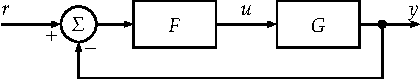
\includegraphics{feedback}
  \caption{\label{fig:feedback}%
    A simple illustration in a floating \envname{figure} environment.  Note that figure captions are always placed under the corresponding figure, and hence that the caption code should always appear at the end of the \envname{figure} environment.}
\end{figure}

\section{Hyperlinks}
%
For readers our the electronically published version of your thesis, as well as yourself while your are working on it, it is very convenient to have working hyperlinks in the document.

\subsection{Basic setup}
%
Basically, hyperlinks are obtained by using the \styname{hypreref} package. However, this package has quite a lot of compatibility issues with other packages, and knowledge about how to deal with these issues is coded into the \rtthesis class.  That is, all you should have to do to get hyperlinks in your document is to specify the \classoption{hyperref} option to \rtthesis.  The class options related to the linking infrastructure of the document are listed in \tableref{tab:hyperref}.

At the time of writing \rtthesis does not call \texcommand{hypersetup} with information about document title, keywords, and other information provided to \texcommand{setupThesis} (see \tableref{tab:setupThesis}).  If someone wants this, it shouldn't be hard to do.

\begin{table}[tbp]
  \centering
  \caption{\label{tab:hyperref}%
    Class options related to (hyper) linking infrastructure.}

  \begin{tabular}{l p{0.5\linewidth}}
    \toprule%
    \textbf{Class option} & \textbf{Meaning} \\
    \otoprule%
    \classoption{hyperref} & Turn on hyperlinks using the \styname{hyperref} package.  Default. \\
    \classoption{nohyperref} & Turn off hyperlinks, and compensate for commands no longer provided by the \styname{hyperref} package. \\
    \midrule%
    \classoption{backref} & Turn on bibliography back references.  Default. \\
    \classoption{nobackref} & Turn off bibliography back references.  (Currently required if you plan to use the features of \styname{bibunits}.)\\
    \bottomrule%
  \end{tabular}
\end{table}


\subsection{Hyperlinks and electronic publishing}
%
To make your dear hyperlinks survive all the way to the electronic publishing system, you may have to replace the file that is sent to e-press by LiU-tryck.  The problem is that LiU-tryck creates a compressed version of the file that is used in the printer, and the compression will remove nice features such as page numbers, hyperlinks, and bookmarks.  Fortunately, the guys at e-press seem to be understanding and will accept to publish a file that they receive directly from you.

\subsection{Page number formatting in the index}
%
If you use an index in your thesis, you will often want to change the formatting of certain page numbers in the index.  Without \styname{hyperref}, this could look like
{\verbatimsize
\begin{verbatim}
hyperlinks\index{hyperlinks|textit}
\end{verbatim}}
to get the page number for this occurrence of \emph{hyperlinks} to be typeset in italics.  The problem with this is that this page number will not be a hyperlink, while other page numbers will be hyperlinks to the correct page.  To get both italics and a hyperlink you need to define a special index formatting commands like the following.
{\verbatimsize
\begin{verbatim}
\newcommand{\hyperpageit}[1]{\textit{\hyperpage{#1}}}
\newcommand{\hyperpagebf}[1]{\textbf{\hyperpage{#1}}}
\newcommand{\hyperpagefootnote}[1]{\hyperpage{#1}n}
\end{verbatim}}

Now, you can write
{\verbatimsize
\begin{verbatim}
hyperlinks\index{hyperlinks|hyperpageit}
\end{verbatim}}
to get both italics and a hyperlink.  The \rtthesis class will provide a trivial definition of \texcommand{chapter} in case \styname{hyperref} is not loaded, so you may safely start to use the above definitions even if you are not sure whether you will use hyperlinks in the end.

\subsection{Friendlier hyperlinks}
%
The default mechanism for references in \LaTeX{}, being the command \texcommand{ref}, is modified as expected by the \styname{hyperref} package.  For instance, the number in “chapter~\ref{cha:rtthesis}” is linked to the beginning of the current chapter (if you click it, be sure to just the \emph{jump back} function of your \textsc{pdf} viewer to get back to here!).  However, all of “\hyperref[cha:rtthesis]{this}” is also a link to the same place.  That is, it is possible to other things than the number itself as links.  We could also make a reference that will never be linked, like in “chapter~\ref*{cha:rtthesis}”.

So, what's so friendly about this?  What I'm aiming at is that you can say “\hyperref[cha:rtthesis]{chapter~\ref*{cha:rtthesis}}”.  The code for this link is
{\verbatimsize
\begin{verbatim}
\hyperref[cha:rtthesis]{chapter~\ref*{cha:rtthesis}}
\end{verbatim}}

Of course, it is very annoying to repeat the key twice; first to point the hyperlink to the correct place, second to show the number of the chapter.  With the \texcommand{autoref} command from the \styname{hyperref} bundle, we get “\autoref{cha:rtthesis}”.  This is almost perfect.  The problem is that one cannot get an uppercase initial at the beginning of a sentence without redefining “chapter” to “Chapter“,
{\verbatimsize
\begin{verbatim}
\renewcommand{\Chaptername}{Chapter}
\end{verbatim}}
but then we will not get the nice lower case initial in the middle of a sentence.  Many authors don't bother about this and use uppercase initials irrespectively of where in a sentence the reference appears.

The only solution I (Henrik Tidefelt) knows of, is to define special commands for each type of reference.  A basic solution might look as follows.
{\verbatimsize
\begin{verbatim}
\newcommand{\chapterref}[1]{\hyperref[#1]{chapter~\ref*{#1}}}
\newcommand{\Chapterref}[1]{\hyperref[#1]{Chapter~\ref*{#1}}}
\end{verbatim}}

You should then use \texcommand{chapterref} in the middle of a sentence, and \texcommand{Chapterref} at the beginning of a sentence.  I you later decide that you want to have upper case initials everywhere, you just have to change your definitions to
{\verbatimsize
\begin{verbatim}
\newcommand{\chapterref}[1]{\hyperref[#1]{Chapter~\ref*{#1}}}
\newcommand{\Chapterref}[1]{\hyperref[#1]{Chapter~\ref*{#1}}}
\end{verbatim}}

A more complete solution will also provide commands for the plural forms “chapters” and “Chapters”.

It is also nice to use a similar technique for page references.  For instance, this chapter starts on \hyperref[cha:rtthesis]{page~\pageref*{cha:rtthesis}}, and such links can be created easily using a command like
{\verbatimsize
\begin{verbatim}
\newcommand{\pagepageref}[1]{\hyperref[#1]{page~\pageref*{#1}}}
\end{verbatim}}

Because of the many possible preferences for how to handle labels and references within documents, \rtthesis does not define any related commands.  The current section should give you some ideas of what can be achieved, and now it is up to you to design your own solution or borrow a solution from someone else (or simply stick with \texcommand{autoref} or the 1980's way of doing things)!

\section{Backreferences from the bibliography}
%
By default, \rtthesis uses the \styname{backref} package to put references from the bibliography back into the text.  The options for turning this feature on and off are listed in \tableref{tab:hyperref}.

By controlling this feature via the class, the choice whether to use it or not can be made orthogonal to the choice of whether to use \styname{hyperref} or not.

In addition to just loading \styname{backref}, \rtthesis will do a basic setup of the commands used to typeset the list of page numbers for each reference.  This behavior can easily be redefined without modifying the \rtthesis class file.  See the \styname{backref} documentation for details on how to do this!

\section{Using the \styname{bibentry} package}\label{sec:rtthesis:bibentry}
%
The \styname{bibentry} package makes it possible to use the information in the bibliography to present your publications at any place in the document.  In order to work independently of whether you use back references from the bibliography or not, you need to follow the pattern below each time you use the \texcommand{bibentry} command, where \texttt{KEY} is the same key to you publication that you would with use with any other citation command.

\begin{minipage}{1.0\linewidth}
  \verbatimsize
\begin{verbatim}
\begin{quotation}
  \nocite{KEY}\noindent
  \backrefparscanfalse\bibentry{KEY}.\backrefparscantrue
\end{quotation}
\end{verbatim}
\end{minipage}

To use the \envname{quotation} environment is just a suggestion — it will make the reference stand out by using a some what shorter text line width.  Note the period that follows the \texcommand{bibentry} command — the command leaves it up to you how to terminate the entry.  The \texcommand{nocite} command ensures that the reference appears in the bibliography, which is necessary to produce the entry.  The \texcommand{noindent} commands simply prevents the first line in the \envname{quotation} from being indented.  The commands \texcommand{backrefparscanfalse} and \texcommand{backrefparscantrue} are related to the \styname{backref} package used to produce back references from the bibliography, and should always surround the \texcommand{bibentry} command.  In case you have turned back references off using the \classoption{nobackref}, \rtthesis will provide substitutes for these two commands.


\section{Fonts}
%
Though basically not a task for a \LaTeX{} class, \rtthesis will assist in loading some font packages.  There are some class options that control this behavior, described below, and if these options are not good enough for you, you may have to make your own copy of the class and replace the font packages you don't like.  Options for font selection are listed in \tableref{tab:fonts}.

One reason, however, for letting \rtthesis handle the font selection is that this makes it possible for the class to do some things more intelligently.  At the moment, \rtthesis will help you make use of some of the goodies of KpFonts, if you choose to use that font.

\begin{table}[tbp]
  \centering
  \caption{\label{tab:fonts}%
    Class options related to fonts.  When slanted small caps are activated, theorem-like environments will use slanted text instead of italics.  The lower part of the table are examples of options that will be understood by the \styname{kpfonts} package, and are only meaningful in combination with the \classoption{kp} option.  (Note that options passed to \rtthesis, but that are not understood by \rtthesis will be passed on automatically by \LaTeX{} to loaded packages.)}

  \begin{tabular}{l p{0.5\linewidth}}
    \toprule%
    \textbf{Class option} & \textbf{Meaning} \\
    \otoprule%
    \classoption{kp} & Use KpFonts (Kepler) and activate slanted small caps.  Default.\\
    \classoption{times} & Use Times and deactivate slanted small caps.\\
    \classoption{lm} & Use Latin Modern and deactivate slanted small caps.\\
    \midrule%
    \classoption{largesmallcaps} & Let the small caps be slightly higher than an \emph{x}.  See the KpFonts documentation!\\
    \classoption{intlimits} & Placement of integration limits.  See the KpFonts documentation!\\
    \classoption{widermath} & Put just a little more horizontal space between entities in math mode.  See the KpFonts documentation!\\
    \bottomrule%
  \end{tabular}
\end{table}

\section{Hanging punctuation}
%
The \rtthesis class automatically loads the \styname{pdfcprot} package with its default settings.  It uses a pdf\TeX{} feature to make punctuation hang into the right margin.  If you don't like it, make your own copy of the class and comment out the line that loads the package.  One reason not to use it would be if your document will be (perhaps only occasionally) typeset using the old \TeX{} program, since this will lead to noticeable differences in the line breaks compared to when pdf\TeX{} is used.  No matter what you choose, make your choice \emph{before} you start working with the page breaks in your document!

\section{Paragraph breaks}
%
There are two common ways of visualizing paragraph breaks in a document, illustrated by the two examples below.  The look of paragraph breaks is controlled using the class options listed in \tableref{tab:parskip}.

\begin{table}[tbp]
  \centering
  \caption{\label{tab:parskip}%
    Class options related to formatting of paragraph breaks.}

  \begin{tabular}{l p{0.5\linewidth}}
    \toprule%
    \textbf{Class option} & \textbf{Meaning} \\
    \otoprule%
    \classoption{noparskip} & US style, see \exampleref{ex:paragraph-break-noparskip}.  Default.\\
    \classoption{parskip} & European style, see \exampleref{ex:paragraph-break-parskip}.\\
    \bottomrule%
  \end{tabular}
\end{table}

% \begin{example}[Default text]
%   This example does not mess with the lengths controlling the paragraph break format.  But you bet it ends in vmode!

% \end{example}

% It is good to see what it looks like if one puts text just below an example.

% \begin{example}[Default text]
%   This example does not mess with the lengths controlling the paragraph break format.  This one ends in hmode!
% \end{example}

\begin{example}[Indented first line]\label{ex:paragraph-break-noparskip}%
  \setlength{\parskip}{0pt}%
  \setlength{\parindent}{1.5em}%
  This style is still the most common.  It is particularly dominant in text written in the US.

  It is a matter of style whether to omit the indentation of the first line after a sectioning command such as \texcommand{chapter} or \texcommand{subsection}.  The omission is typically automated, but can also be enforced using the  \texcommand{noindent} command.

  One drawback of not having vertical space between paragraphs is that it will be harder for pdf\TeX{} to find good places for page breaks, compared to the option shown below.  If you like compact documents, however, this is the option for you!

  For testing purposes, this example ends with a paragraph break, so that \TeX{} is in \emph{vmode} at the end.  You should always avoid this, but the class will try to compensate for your mistakes\ldots

\end{example}

\begin{example}[Vertical white space]\label{ex:paragraph-break-parskip}%
  \setlength{\parskip}{1ex}%
  \setlength{\parindent}{0pt}%
  This style is still increasing in popularity.  It is rather common in modern texts written in Europe, and the style has received special attention from the Netherlands \TeX{} user group \emph{Nederlandstalige \TeX{} Gebruikersgroep, \textsc{ntg}}.  Their efforts can be used through their variants of the standard \LaTeX{} classes.

  Unfortunately, the \textsc{ntg} classes are not compatible with \rtthesis, and the solution provided by the \styname{parskip} package is only part of the solution.  Hence, \rtthesis will do more than just loading the \styname{parskip} package for you if you specify the \classoption{parskip} option.

  A good reason to put code related paragraph breaks in the class file is that all the small adjustments that different people come up with can be put in one placed so that they are accessible to future users of the class.
\end{example}

\section{Page breaks}\label{sec:tipt:page-breaking}
%
There is a whole lot to say about how to obtain nice page breaks.  You will find some recommendations below, but do not use this document as your ultimate reference on this topic!  (This document itself contains some really nasty page breaks --- at least at the time of writing this --- as a result of not paying any attention at all to the problem.  It would simply bee too time-consuming to keep adjusting the page breaks each time the document is edited.)
\begin{itemize}
\item
  Take no consideration of page breaks until page breaking is the only aspect of your thesis that remains to be taken care of!  Page breaking involves a lot of manual intervention of the automatic mechanisms in pdf\TeX{}, and as soon as you have started to intervene, any further changes to the text will risk to ruin your page breaking fixes, and may even lead to worse results than before since the automatic page breaking has been tampered with.
\item
  First thing to try is to make changes to the text to help the automatic page breaking mechanism.  Try to make sentences longer or shorter depending on the situation.  Since this will not tamper with the automatic page breaking mechanism, this option will incur the least loss of maintainability of your document.
\item
  Can the location of floats be changed to improve page breaks?  Play around with exactly where in your source files the code for the floating environments appears!
\item
  You may also try to force early page breaks using the \texcommand{Needspace*} command.  For instance, putting
{\verbatimsize
\begin{verbatim}
\Needspace*{2\baselineskip}
\end{verbatim}}
before a paragraph will cause a page break if there is not enough vertical space on the page to hold two lines of text.  The good thing about this option is that your intervention will cause no harm if the \texcommand{Needspace*} command appears in the middle of a page.  The bad thing about this option is that it may cause remaining vertical space on the broken page to be stretched quite badly.  You should always check that the resulting page looks OK!

For more information, and related commands, see the documentation for the \styname{needspace} package!
\item
  The last option is to play with the vertical size of individual pages.  For instance, putting
{\verbatimsize
\begin{verbatim}
\enlargethispage{2\baselineskip}
\end{verbatim}}
before a paragraph you would like to fit into the current page will make space for two extra lines of text.  This avoids the bad stretching of vertical space that the \texcommand{Needspace*} option may cause.  However, if you would make other changes that makes tampering with the page size unnecessary, it will be very time-consuming to detect this and remove the no longer needed \texcommand{enlargethispage} command.
\end{itemize}

Note that manual page breaking is a time-consuming task.  Make sure to have at least one full day allocated to page breaking before you submit your thesis for print!

\section{Input encoding}
%
Two input encodings are supported, being \mbox{latin-1} and \mbox{\textsc{utf}-8}.  The choice of input encoding should be made via the \rtthesis class, so that the class can use the correct encoding to define certain global strings.  The input encoding options are listed in \tableref{tab:inputenc}.

\begin{table}[tbp]
  \centering
  \caption{\label{tab:inputenc}%
    Class options related to input encodings.  Note that there is no default; \rtthesis requires one of these options to be passed explicitly.}

  \begin{tabular}{l p{0.5\linewidth}}
    \toprule%
    \textbf{Class option} & \textbf{Meaning} \\
    \otoprule%
    \classoption{latin1} & Simply use \styname{inputenc} with option \classoption{latin1}. \\
    \classoption{utf8} & Use \styname{inputenc} with option \classoption{utf8}, and define some additional characters. \\
    \bottomrule%
  \end{tabular}
\end{table}

Choose \mbox{latin-1} if you depend on lots of files using this encoding, and do not want to change the encoding of these files.  Changing the encoding of a file is easy both in Emacs and using the \emph{iconv} command line utility.  The \mbox{latin-1} encoding is the default in \rtthesis, but the choice can be made explicit by passing the \classoption{latin1} option to the class.

Choose \mbox{\textsc{utf}-8} to be able to type many more characters directly in your \LaTeX{} sources compared to \mbox{latin-1}.  For instance, names of foreign authors often use characters that cannot be entered directly using \mbox{latin-1}.  In \mbox{\textsc{utf}-8}, most of these as well as special punctuation characters such as double quotes and various dashes can be entered directly in the source.  Use the \classoption{utf8} class option if your files are encoded in \mbox{\textsc{utf}-8}.

The current implementation of \mbox{\textsc{utf}-8} in the \styname{inputenc} package only defines the input encoding for characters that have corresponding glyphs in active fonts (see the \styname{inputenc} documentation for details).  This means that some characters that \TeX{} would build by combining several glyphs will not be defined by \styname{inputenc}.  If the \classoption{utf8} is given, \rtthesis will define a list of additional characters by inclusion of the package \styname{rtthesis-utf8-ext}.  If you need additional characters, you should make your own package similar to \styname{rtthesis-utf8-ext}, and then let the maintainer of \rtthesis know, so that the additional characters may be added to \styname{rtthesis-utf8-ext} so that others can use them in the future.  Note that \styname{rtthesis-utf8-ext} may be a useful package also when you are not using the \rtthesis class.

It is easy to set up Emacs so that it uses the \mbox{\textsc{utf}-8} encoding for your \TeX{} files, but it is out of the scope of the current document to give further explanations here.


\section{\rtthesis and \styname{natbib}}
%
Interoperability with different bibliography packages is a tricky issue.  It has been a design decision to try to support at least \styname{natbib}, at the cost of loosing compatibility with other packages such as \styname{jurabib}.  The core of the problem is package loading order, requiring \styname{natbib} to be loaded very early on in the class.  To pass options to \styname{natbib}, pass them as global class options to \rtthesis.  Note that the default options for \styname{natbib} are quite reasonable, and see \tableref{tab:natbib} for examples of other options that \styname{natbib} will pick up.  If you know how to resolve the conflict with the \styname{natbib} option \classoption{usebibunits}, let the \rtthesis maintainer know!

\begin{table}[tbp]
  \centering
  \caption{\label{tab:natbib}%
    Class options related to the \styname{natbib} package.  Note that options can be passed to \styname{natbib} by passing them as global class options to \rtthesis.  See the \styname{natbib} documentation for more useful options.}

  \begin{tabular}{l p{0.5\linewidth}}
    \toprule%
    \textbf{Class option} & \textbf{Meaning} \\
    \otoprule%
    \classoption{authoryear} & Default option of \styname{natbib} --- no need to specify.\\
    \classoption{round} & Default option of \styname{natbib} --- no need to specify.\\
    \classoption{colon} & Default option of \styname{natbib} --- no need to specify.\\
    \midrule%
    \classoption{square} & Example of option that \styname{natbib} will pick up (alternative to \classoption{round}).\\
    \classoption{comma} & Example of option that \styname{natbib} will pick up (alternative to \classoption{colon}).\\
    \midrule%
    \classoption{numbers} & Conflicting \styname{natbib} option --- forbidden in combination with \classoption{usebibunits}, see \classoption{forcenumbers} below.\\
    \classoption{forcenumbers} & Enforce option \classoption{numbers} to be passed to \styname{natbib} (alternative to \classoption{authoryear}) --- it's up to you to resolve the conflict.\\
    \bottomrule%
  \end{tabular}
\end{table}


\section{The lists of previous theses}
%
The lists of previous licentiate's and PhD theses can be found in \textfilename{liclist.tex} and \textfilename{phdlist.tex}, respectively, and the appropriate one of the is automatically included at the end of your thesis.  Both files are found in the directory\\
\textfilename{\$TEXMFGROUPLOCAL/tex/latex/rt/rtthesis} .

Note that it is \emph{your responsibility} to make sure that your thesis is added to the appropriate list after you have sent it to print but before the next thesis of the same kind is printed.  If other people are writing theses at the same time as you, you will have to coordinate your moves in order to make sure that the lists get updated in the correct order.  To get your thesis added to the appropriate list, you simply send an email with information about your thesis to the \rtthesis maintainer.  The information shall be in one of the following formats:

{\verbatimsize
\begin{verbatim}
\licitem{J.~Doe}{Title}{Thesis No}{YYYY}
\end{verbatim}}

or

{\verbatimsize
\begin{verbatim}
\phditem{J.~Doe}{Title}{Theis No}{YYYY}{ISBN}
\end{verbatim}}

It is a good idea to make a copy of the file you need when it is time to print.  If you don't make a copy, and then compile your thesis again at a later time, the list will be wrong because it will include at least one thesis that wasn't prior to yours — namely your own!


\section{Compilation theses}
%
The \rtthesis class aims to support the production of both monographs and compilation theses.  There is a compilation thesis example included with \rtthesis.  Please have a look at that while reading the sections below!


\subsection{Including publications in your thesis}
%
It is assumed that included publications shall be compiled together with the rest of your thesis, as opposed to being included as exactly the way the look where published.  Under this assumption, it is reasonable to expect things such as a suitable chapter numbering, and that the global table of contents includes the sections withing publications.  Note that it would be rather difficult to get things such as the table of contents and other infrastructure right if publications were to be included by direct \textsc{pdf} inclusion.

The \envname{papers} environment provided by \rtthesis will redefine commands and set up some additional commands to support the inclusion of \LaTeX{} sources of your publication.  It is recommended that the environment is placed in a second part of the thesis.  Inside the environment, the \texcommand{chapter} command is redefined to both start a new chapter and set up the title of the publication to be included in the same chapter.  Chapters will be labeled with letters instead of numbers, so it is up to you to make a clear distinction between referencing an appendix chapter and a publication chapter.

If the title of a publication is too long to fit in the page header, you may follow the \texcommand{chaptermark} command by a \texcommand{chaptermark} command.  Since the \texcommand{chaptermark} command takes an optional argument to be used in the table of contents, there are three different variations of the publication title that can be defined.

The word for publications used by \rtthesis is \emph{paper}; it will appear both on the chapter title page and in page headers.  To change this to something else, you simply have to redefine \texcommand{chaptername} to something else inside the \envname{papers} environment.

After setting up the publication title, the \texcommand{author} command should be used to set up the list of authors.  It works as usual, but sports two special \rtthesis commands that should be used when there are two author affiliations;  put \texcommand{authorleft} immediately after author names who's affiliation should appear to the left below the list of authors, and put \texcommand{authorright} after the other authors.  There is currently no support for more than two different affiliations.

In case there is only one affiliation, that affiliation is given by \texcommand{paperaffiliation} (which should be set once and for all to your own affiliation), and you use the \texcommand{email} command to specify the list of email addresses to the authors.

In case of two affiliations, you call the commands \texcommand{affilblockleft} ,\texcommand{affilblockright}, \texcommand{emailleft}, and \texcommand{emailright} with the appropriate arguments.  Note that one of the two affiliation block arguments should simply be \texcommand{paperaffiliation}.

Additional information about the publication is given in after \texcommand{item} commands inside the \envname{paperinfo} environment.  In addition to the items given, the environment automatically starts with one item displaying the author information (without any marks related to affiliation blocks).  Three commands are defined by \rtthesis to simplify consistent formatting of additional information.
\begin{itemize}
\item \texcommand{paperedited{\emph{bib-key}}} — For ordinary publications.  The extent to which the publication has been edited should be state clearly.  The bibliography entry will be formatted using the technique described in \sectionref{sec:rtthesis:bibentry}.
\item \texcommand{paperprelver{\emph{ISY-report-number}}} — For publications for which there is only a preliminary version available.  The preliminary version should be published as a technical report at the department, and as no bibliography keys are involved, the technical report will not be listed in any the bibliography.
\item \texcommand{papertechrep{\emph{ISY-report-number}}} — For publications that are not yet even preliminary versions of something.  These too should be published as technical reports at the department, and will not appear in the bibliography.
\end{itemize}

At this point the chapter title page will be finished.   The next step is to make a nice title and abstract for your publication on the following odd page.  Use \texcommand{maketitle} or \texcommand{maketitletwoaffil} depending on whether you set up one or two affiliation blocks.  Then put the publication abstract inside the \envname{abstract} environment.

After this point, you should just be able to include the source of your publication, with \texcommand{section} as the topmost sectioning command (since the publication itself is a chapter of your thesis).

Finally, you must decide where your references should go.  Should there be one global bibliography for the whole thesis, or should there be one bibliography for each publication.  This is the topic of the next section.

\subsection{Compilation theses and bibliographies}
%
If you are fine with having just one global bibliography for the whole thesis, everything should work out of the box.  Hence, this section will try to describe how to do in order to get one bibliography for the background part of your thesis, and one for each publication.

The \rtthesis class only supports this by relying on the \styname{bibunits} package.  Due to package loading order issues, it should always be loaded by passing \classoption{usebibunits} to \rtthesis.  Note that some of the \styname{bibunits} commands appears to be incompatible with bibliography back references, so you need to pass the \classoption{nobackref} to \rtthesis if you plan to use the \styname{bibunits} features.

\begin{remark}
  There is a very interesting package called \styname{biblatex} which is currently in beta version.  Hopefully, it will let us drop the messy packages \styname{bibunits} and \styname{backref}.  You are invited to try this package, and if you find it to work satisfactory it should probably be incorporated in \rtthesis.  Future maintainers of \rtthesis are strongly encouraged to find out what \styname{biblatex} can do for us!
\end{remark}

Use the command \texcommand{defaultbibliography} to specify the bibliography files to use for all of the per-publication bibliographies, and use \texcommand{defaultbibliographystyle} to select the bibliography style, see the \styname{bibunits} documentation for details.

To get an individual bibliography for a publication, you should just have to include that chapter in a \envname{bibunit} environment, and call \texcommand{putbib} where you want the bibliography to appear.  Here, the \texcommand{putbib} command will be redefined by \rtthesis in order to make the bibliography appear in the table of contents.

A bibliography for references that appear in the background part of your thesis are produced as usual with the \texcommand{bibliography} command.  (It might be good to know that \rtthesis will automatically issue the \texcommand{nobibliography*} command in order to make the \styname{bibentry} package work as you would expect.)

\section{Master's theses}\label{sec:msc}
%
The \styname{liuthesis} class by Gustaf Hendeby was developed for the production of master's theses at Linköping University.  The class knows how to create the special pages required by several departments, and in the summer of 2011 this capability was merged into \rtthesis.  This makes it convenient to produce a master's thesis at Linköping University using \rtthesis instead of \styname{liuthesis}, allowing a wider audience to benefit from the more active development of \rtthesis.\footnote{The \LaTeX{} class files tend to be maintained by PhD students, and PhD students have a tendency to be more interested in maintaining the class files for writing licentiate's and PhD theses than class files for master's theses.}

This section describes how to use \rtthesis to produce a master's thesis.  To begin, pass \emph{msc} as the value for the key \emph{type} in the call to \texcommand{setupThesis}, and select your department using the key \emph{department}.  More details are given below, and the reader is encouraged to study the bundled example in order to get a better overall picture.

\subsection{Master's thesis setup}
%
In addition to the pieces of information given to \texcommand{setupThesis} for licentiate's and PhD theses (see \tableref{tab:setupThesis}), there are some that only apply to master's theses.  These are listed in \tableref{tab:setupThesis-msc}.

\begin{table}[tbp]
  \centering
  \caption{\label{tab:setupThesis-msc}%
    \texcommand{setupThesis} key-value pairs for master's theses, in addition to those listed in \tableref{tab:setupThesis}.  Note that values that include white space are surrounded by braces.}

  \begin{tabular}{>{\ttfamily}r !{\texttt{=}} >{\ttfamily}l l}
    \toprule%
    \textbf{Key} & \textbf{Example value} & \textbf{Comment} \\
    \otoprule%
    swetitle & \{Svensk titel\} & Title in Swedish\\
    swesubtitle & \{Bra grejer\} & Optional Swedish subtitle\\
    month & 4 & \\
    day & 9 & \\
    subject & reglerteknik & \\
    site & \{Bosses AB i Linkan\} & \\
    division & \{Avdelningenrt\ldots\} & \\
    department & isy & See \tableref{tab:department} \\
    examiner & \{Lena Lärare\ldots\} & Details given below \\
    supervisor & \{Doktorand Si\} & Details given below \\
    keywords & \{this, that\} & Appears on library page \\
    isrn & LiTH-ISY-EX\ldots & See below \\
    url & \{http://\ldots\} & Thesis download \textsc{url}, see below \\
    \bottomrule%
  \end{tabular}
\end{table}

The value for the key \emph{department} must be one of the special values listed in \tableref{tab:department}.  This setting controls both the department name and address, as well as how the special pages of the thesis are formatted.  Please help the \rtthesis maintainer to keep the special pages for your department up to date.

In the values for the keys \emph{examiner} and \emph{supervisor}, multiple persons should be separated using \texcommand{AND}, and the affiliation of a person should appear after \texcommand{AT}, like this:
{\verbatimsize
\begin{verbatim}
  supervisor={Doktorand Si \AT \textsc{isy}, Linköpings universitet
         \AND Ingenjör Så \AT Företaget},
\end{verbatim}}

The \textsc{isrn}\footnote{The \textsc{iso} standard for \textsc{isrn} was withdrawn in 2007, but the report numbering system is still in use at Linköping University.} should be something like
{\verbatimsize
\begin{verbatim}
  isrn=LITH-ISY-EX-{}-YY/NNNN-{}-SE
\end{verbatim}}
but the format varies between different departments.  Note that if the report identifier contains two or three consecutive dashes, they have to be separated by empty braces in the input to prevent \LaTeX{} from interpreting them as one character.  The thesis download \textsc{url} should be something like
{\verbatimsize
\begin{verbatim}
  url={http://urn.kb.se/resolve?urn=urn:nbn:se:liu:diva-XXXXX}
\end{verbatim}}
The exact details regarding the report number and \textsc{url} will be given to you by the librarian when you register your thesis.

\begin{table}[tbp]
  \centering
  \caption{\label{tab:department}%
    Recognized values for the key \emph{department} in \tableref{tab:setupThesis-msc}.}

  \begin{tabular}{>{\ttfamily}c p{0.45\linewidth} l}
    \toprule%
    \textbf{department} & \textbf{Department of\ldots} & \textbf{Updated}\\
    \otoprule%
    ida & Computer and Information Science & Not after 2008-08-01\\
    ifm & Physics, Chemistry and Biology & 2011-07-03\\
    iei & Management and Engineering & \emph{Out of date!}\\
    isy & Electrical Engineering & 2011-07-03\\
    itn & Science and Technology & 2011-07-03\\
    mai & Mathematics & 2011-07-03\\
    \bottomrule%
  \end{tabular}
\end{table}

\subsection{Special pages}
%
The requirements on a master's thesis include that certain information go on the front page and title page of the thesis.  Further, a library page for cataloging purposes is required at the beginning of the thesis, and a page with copyright information is required at the end.  The copyright page is automatically added at the end.  The other special pages can be produced using the macros \texcommand{makeFrontPage}, \texcommand{maketitle} (as usual), and \texcommand{makeLibraryPage}.  These macros are meant to be invoked more or less immediately after \texcommand{begin\{document\}}, see the bundled example for details.  Note that in the printed report, the front page should be replaced by the cover, and the library page is \emph{probably} meant to be on a loose piece of paper inserted between the cover and the title page.

There is no magic that puts the correct abstract on the library page, but the abstract must be given as an argument to \texcommand{makeLibraryPage}.  To make sure that this is exactly the same as the abstract in the thesis, it is recommended that you write the abstract text without any surrounding \envname{abstract} environment in a separate file, say \textfilename{svensk-sammanfattning.tex}.  Then you can use this file twice, like this:
{\verbatimsize
\begin{verbatim}
\makeLibraryPage{\input{svensk-sammanfattning}}

\begin{abstract}[swedish]
  \input{svensk-sammanfattning}
\end{abstract}
\end{verbatim}}
(The bundled example uses this technique.)

\subsection{Choice of language}
%
If your main report language will be Swedish, put
{\verbatimsize
\begin{verbatim}
\selectlanguage{swedish}
\end{verbatim}}
right after
{\verbatimsize
\begin{verbatim}
\begin{document}
\end{verbatim}}
Also make sure to provide the thesis title (and possibly subtitle) in Swedish via the keys \emph{swetitle} and \emph{swesubtitle} to \texcommand{setupThesis}.  You may then omit writing an abstract in English.

If your main report language will be English you don't need to change the default choice of language.  However, you must provide a thesis title both in English and Swedish, and the thesis should contain abstracts in both English and Swedish.


\section{Compiling the document}
%
Using all the current features of \rtthesis, the following sequence of steps is usually sufficient to compile your document.  Let us assume your main file is named \textfilename{main.tex}.
\begin{itemize}
\item
  First run
{\verbatimsize
\begin{verbatim}
pdflatex main
\end{verbatim}}
  to scan your document for references, labels, and index items.
\item
  Then run
{\verbatimsize
\begin{verbatim}
bibtex main
\end{verbatim}}
  to extract relevant references from your bibliography file(s).  If you are using the \styname{bibunits} package, you also have to process some additional files;
{\verbatimsize
\begin{verbatim}
bibtex bu1; bibtex bu2; ...; bibtex bun
\end{verbatim}}
\item
  If you have an index in your document, run
{\verbatimsize
\begin{verbatim}
makeindex main
\end{verbatim}}
  to format it.
\item
  Then run
{\verbatimsize
\begin{verbatim}
pdflatex main
\end{verbatim}}
  to insert references in the typeset document.  This will typically move things around, and your page references will be invalidated.
\item
  Hopefully, it is enough to run
{\verbatimsize
\begin{verbatim}
pdflatex main
\end{verbatim}}
  once more now to get the page references right.  You will get a warning if you need to repeat this step.
\end{itemize}

In addition to the steps above, certain auxiliary files must be deleted when certain features of the class are turned on or off.  In particular, turning hyperlinks on or off requires the following.
{\verbatimsize
\begin{verbatim}
rm main.aux main.toc main.ind
\end{verbatim}}

\section{Generating a thesis cover and the “spikblad”}
%
A thesis cover can be created by making a file that contains the \texcommand{makecover} command.  For example, given that \textfilename{mythesis.sty} invokes the \texcommand{setupThesis} command with the necessary information (see \tableref{tab:setupThesis}), a PhD thesis cover can be made as follows.

\begin{minipage}{1.0\linewidth}
  \verbatimsize
\begin{verbatim}
\documentclass[utf8,phd]{rtthesis}
\usepackage{mythesis}

\makecover
\end{verbatim}
\end{minipage}

Note that while all licentiate's theses should have the same cover, there is no standard (but many rules set by the university!) for the PhD theses.  The \texcommand{makecover} command gives a “classic” cover that quite a few people have used over the years.  This cover might also be useful as a means to compile the information needed when LiU-Tryck (or some other printing company) designs a more artistic cover.

For a dissertation, there should always be a “spikblad” (literally, \emph{nailing sheet}).  Such an information sheet can be generated easily if the English abstract is put in a separate file.  In this case, the same abstract can be included both in the thesis and in a separate file that defines the “spikblad”.  For a licentiate's thesis presentation, a similar information sheet should be produced.  The monograph example demonstrates how to created these, see the files \textfilename{spikblad.tex} (for dissertations) and \textfilename{licinfo.tex} (for licentiate's thesis presentations).


\section{Required logotypes (not included with \rtthesis)}
%
\Tableref{tab:logos} lists files with logotype graphics that are needed by \rtthesis.  They are not part of the \rtthesis bundle since they are used in many other contexts as well.  Users at the Division of Automatic Control should have access to these files via the group's common texmf tree, but in order to be able to work at home you will have to make sure one way or another that the files are installed.

Beware that the university changes logos quite often. Make sure that there are no new versions of the logos you use.  If the logos are old, please, let the \rtthesis maintainer know so that the files get updated at the central location.

\begin{table}[tbp]
  \centering
  \caption{\label{tab:logos}%
    Files with logotype graphics used by \rtthesis.  Use the command \texttt{kpsewhich} to find where the files are located!}

  \begin{tabular}{l p{0.5\linewidth}}
    \toprule%
    \textbf{Filename} & \textbf{Use} \\
    \otoprule%
    \textfilename{LinkUniv\usc{}sigill\usc{}sv.pdf} & For the cover and the first page in PhD theses.\\
    \textfilename{LiTH\usc{}staende\usc{}eng\usc{}sv.pdf} & For the cover of both licentiate's and PhD theses.\\
    \textfilename{rtlogo\usc{}tall.pdf} & For the first page in licentiate's theses.\\
    \bottomrule%
  \end{tabular}
\end{table}

\section{Compatibility with standard packages}
%
Incompatibilities between different packages is a problem that quickly becomes quite an issue when the list of packages used in a document grows beyond just a few.  It may sound strange, but it is because of compatibility problems that \rtthesis includes a rather long list of packages for you.  The reason is that this allows knowledge about package loading order requirements and various workarounds, to be encoded in the class file.

No list of packages included by \rtthesis will be presented here, but you should check the class file directly to be sure that you always get the correct answer to whether a package is included or not (or you can just read the compilation output).

Packages with no known compatibility issues will generally not be included by \rtthesis unless needed by the class itself.  The following list contains some examples of useful packages that are not included by \rtthesis.  They \emph{should} be compatible with \rtthesis.  Please let the \rtthesis maintainer know if any of these are no longer compatible, or if you have suggestions for other packages that should be mentioned here.
\begin{itemize}
  \item \styname{nextpage} — page break control
  \item \styname{algorithm} — code listings
  \item \styname{listings} — code listings
  \item \styname{SIunits} — physical dimensions
  \item \styname{pmat} — partitioned matrices
  \item \styname{bm} — bold math
  \item \styname{footmisc} — extras for footnotes
  \item \styname{dcolumn} — decimal point alignment in tables (the already included \styname{array} can also do this)
  \item \styname{lettrine} — start chapter with fancy letter
  \item \styname{supertabular} — multi-page tables
  \item \styname{longtable} — multi-page tables
  \item \styname{multirow} — tabular entries occupying more than one row
\end{itemize}



\backmatter
\small
%\bibliographystyle{plain}
\bibliography{BibTeX/Cite-General,BibTeX/Cite-Growth,BibTeX/Cite-PL,BibTeX/Cite-Solar,BibTeX/Cite-Watersplitting}
\printindex


\end{document}




